\chapter{Equilibrium Statistics of the Forced Pinned Polymer Loop}
\graphicspath{{Chapter3/Figs/}}

In previous chapter, we introduced the details of our polymer loop model for chromosomes and the simulation techniques. In this chapter, we will investigate the equilibrium statistics of the model and use the results to understand the chromosome alignment in fission yeast. 

In order to tract the model analytically, we will neglect the complex interactions such as bending energy, excluded volume effect and hydrodynamical perturbations. In another word, our model is the simplest freely-jointed polymer loop model. The transferred coordinate is utilized so that the first bead representing SPB is pinned. And an external force field will be applied. 

We will start by introducing the setting of the model in the first section. The equilibrium statistics of 1D and 3D are discussed separately in section two and three. In the fourth section, we discuss of shape of steady pinned polymer loop in external force field. We want to mention here that the work of first three sections were done by close cooperation with Yen Ting Lin. Most of the theory was developed by him and I contribute to all the simulations. 


%********************************** %First Section  **************************************
\section{Pinned polymer loop in a constant force field}
\label{sec:pinned_polymer_loop}
\begin{figure}[htpb]
    \centering
    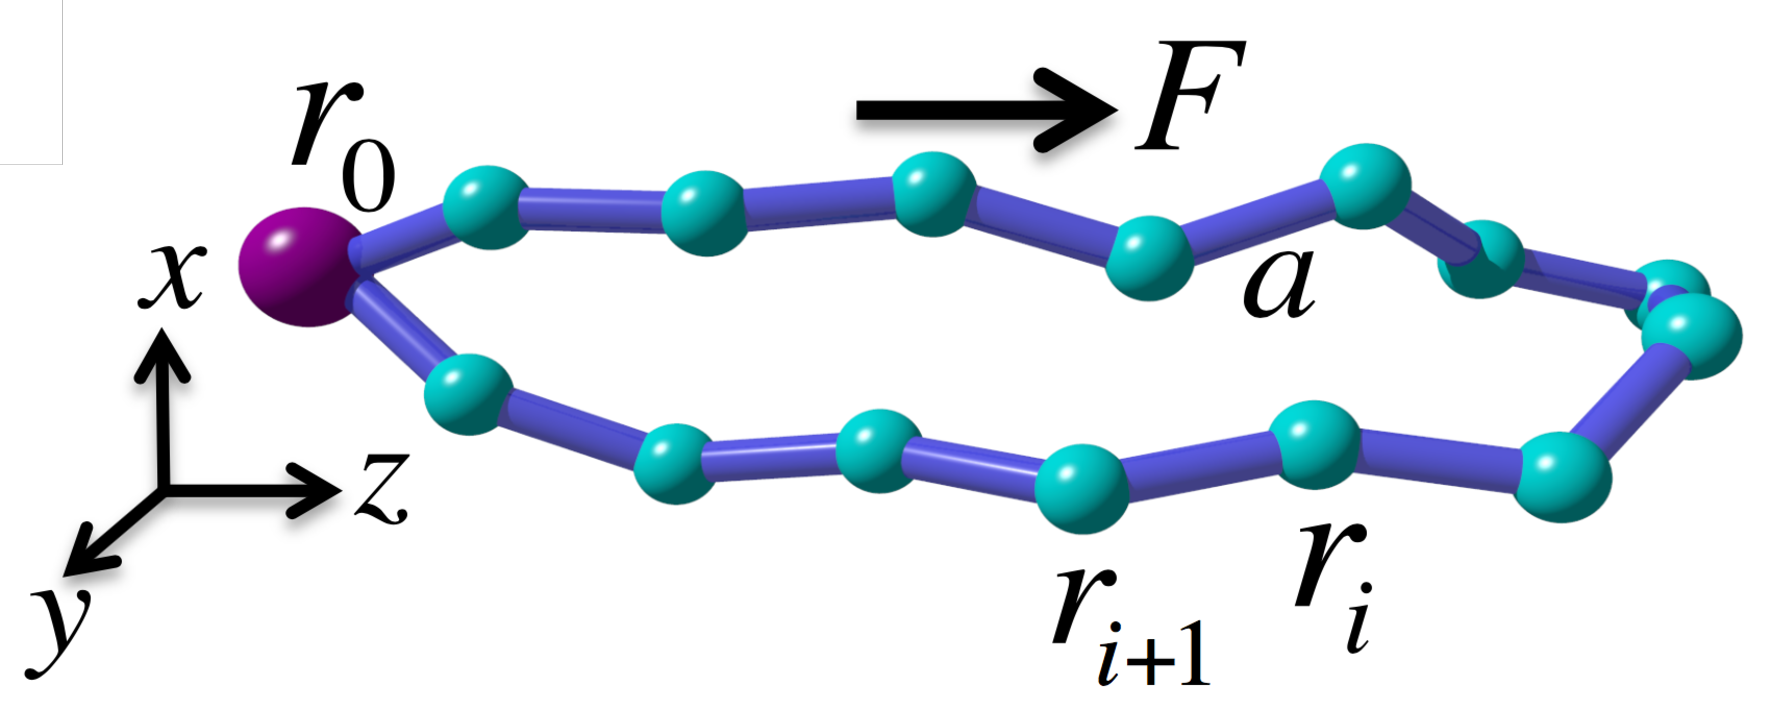
\includegraphics[width=0.7\linewidth]{beadrod}
    \caption{Sketch for the pinned bead-rod loop and notations. }
    \label{fig:beadrod}
\end{figure}

As mentioned in section~\ref{sec:polymer_model_and_dna}, the chromosomes of fission yeast can be considered as pulled polymers with constant velocity during the period of moving towards to one direction. In this case, it is appropriate to discuss the equilibrium statistics as the relaxation time scale is much smaller than the oscillation time scale. Using the coordinate transformation introduced in the section~\ref{sec:stochastic_models_of_polymer_loops}, the pulled polymer loop model can be transferred to pinned polymer loops in constant external force field. We will discuss the equilibrium statistics of the pinned polymer loops in an external force field in this chapter.

Let us first clarify some notations before seeking for the solution. There are $L$ beads (including the SPB) in the loop and the SPB is denoted by $\mathbf{r}_0$ or $\mathbf{r}_L$ in periodic indexing. Without loss of generality, we assume it is pinned to the origin point, i.e. $\mathbf{r}_0 = \mathbf{r}_L = \mathbf{0}$. The length of each rod is $a$. And the constant external force field denotes by $\mathbf{F}$ is in the $z$ direction. The potential energy of the pinned polymer loop can be written as:
\begin{equation}
    \label{eq:energyBeadrod}
    E = E_0 - a\sum_{i=1}^{L} \mathbf{F}\cdot\mathbf{r}_i
\end{equation}
where $E_0$ is assumed to be a constant that denotes configuration independent energy. It is not important for the study of equilibrium statistics, we keep it here just for completeness. The orientation of the $j^{\rm{th}}$ rod is denoted by $\mathbf{u}_j = (\mathbf{r}_{j}-\mathbf{r}_{j-1})/a$. So the $i^{\rm{th}}$ bead position can be written as:
\begin{equation}
    \label{eq:beadposRodsum}
    \mathbf{r}_i = a \sum_{j=1}^{i} {u}_j.
\end{equation}
Plug it into Eq.~\eqref{eq:energyBeadrod}, we arrive at
\begin{equation}
    \label{eq:energyRodsum}
    E = E_0-a\sum_{i=1}^{L}\sum_{j=1}^{i}\mathbf{F}\cdot\mathbf{u}_j.
\end{equation}
Notice that the looping condition indicates
\begin{equation}
    \label{eq:loopCondition}
    \sum_{j=1}^{L} \mathbf{u}_j = 0.
\end{equation}

In the following two sections, we will solve the equilibrium statistics in 1D first and extend the theory to 3D.


%********************************** %Second Section  *************************************
\section{Pinned Polymer Loop in 1D}
\label{sec:pinned_polymer_loop_in_1d}

As the same strategy to study many problems in physics, let us start to solve the equilibrium statistics from the simplest 1D case. The one dimensional polymer is possible because we neglect the exclusion volume effect so that the beads and rods are free to overlap. It is a simple idealized model. We will show in the following that an elegant mapping for the one dimensional pinned polymer loop to a famous classical physical model can be found. 

\subsection{Mapping to a particle system on 1D lattice}
\label{sub:mapping_to_a_particle_system_on_1d_lattice}

The pinned polymer in 1D is very simple. The configuration of the polymer can be specified by the orientation of the rods. In 1D, there are only two possible orientations for all rods, i.e. along the axis or against the axis. 

Let us denote the $j^{\rm{th}}$ rod orientation by $u_j\in\{-1, +1\}$, where $u_j = +1$ means the rod orientates along the axis and $u_j = -1$ means the rod orientates against the axis. Again the $i^{\rm{th}}$ bead position in 1D is $z_i = a\sum_{j=1}^{i}u_j$. Now let us introduce a shifted and rescaled variable 
\begin{equation}
    \label{eq:variableu2n}
    n_j = (u_j + 1)/2. 
\end{equation}
We can easily find that $n_j\in\{0,1\}$. The configuration of the 1D polymer can be denoted by $\{n_1, n_2, \cdots, n_L\}$. Since $n_j$ is a binary variable, we can interpret $n_j = 1$ as a lattice site occupied by a particle, and $n_j = 0$ as an empty lattice site. In this way, we find a one-to-one mapping from the configuration of polymers to particles on lattice sites. See in Fig. \ref{fig:mapping}. The number of rods equals to the number of lattice sites. Without loss of generality, we have shown in the figure the right-orientated rod corresponds to an occupied site, and the left-oriented rod corresponds to an empty site.

\begin{figure}[htpb]
    \centering
    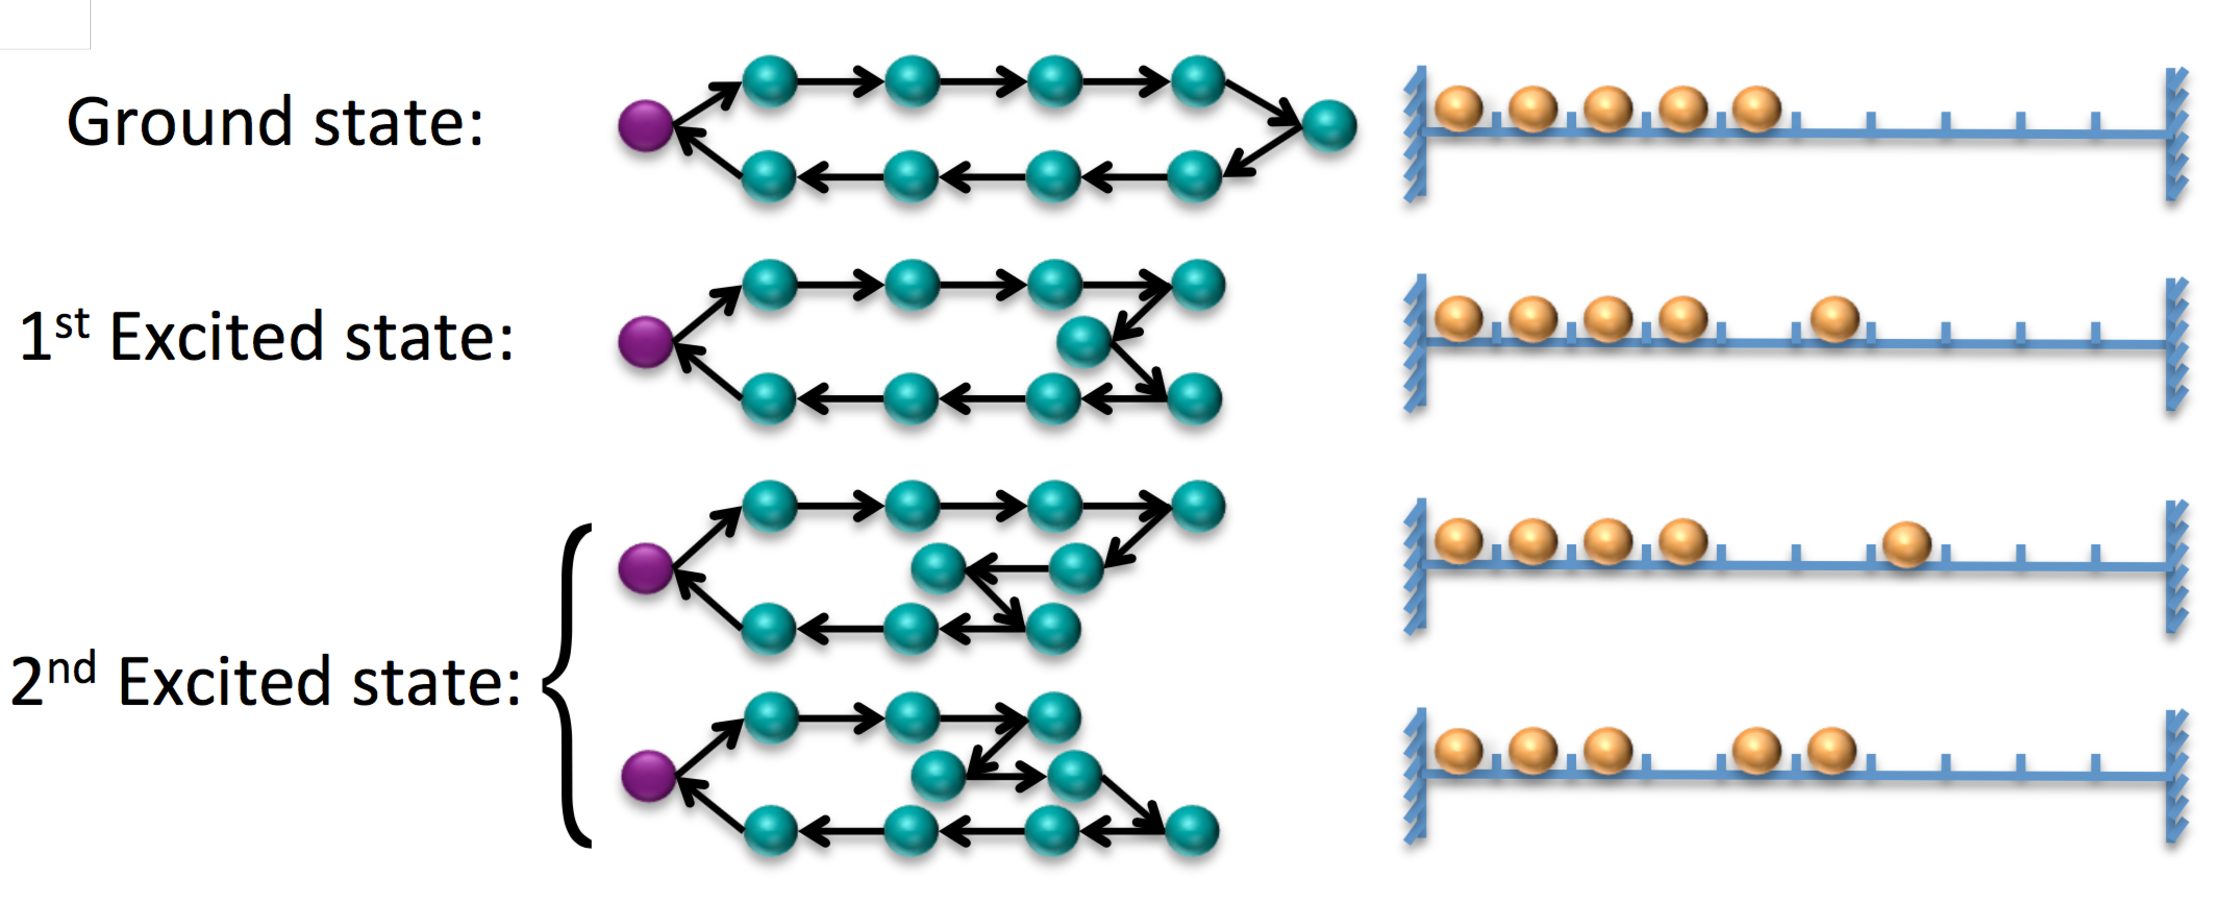
\includegraphics[width=0.9\linewidth]{mapping}
    \caption{Illustration for the mapping from 1D pinned polymer loop to Fermionic particles on 1D lattice sites. }
    \label{fig:mapping}
\end{figure}

Here are some remarks for the mapping:

$\bullet$ The mapped particles are exclusive to each other. It is not possible for one lattice occupied by more than one particles. In another word, these particles are Fermions. This is because the system is a two state system, there is no correspondent polymer state for a site occupied by more than one particle.

$\bullet$ According to the looping condition Eq. \eqref{eq:loopCondition}, the total number of rods pointing to the right must be exact $L/2$. Correspondingly, the total number of particles also must be exact $L/2$, i.e.
\begin{equation}
    \label{eq:loopConditionParticle}
    \sum_{j=1}^{L}{n_j} = \frac{L}{2}.
\end{equation}
Furthermore, the number of particles must be conserved during the change of configurations.

$\bullet$ The dynamics of 1D polymer can be mapped to the particle hopping process on the 1D lattice. This part will be discussed in next chapter.

$\bullet$ The mapping is essentially from a two state system to a two state system. One can also interpret the two state as spin up and spin down or any other two state systems. We use the particle-lattice interpretation because it is familiar and intuitive to most people. 

Now let us discuss the energy of the system. Rewrite Eq. \eqref{eq:energyRodsum} in 1D we get
\begin{equation}
    \label{eq:energyRodsum1D}
    E = E_0 - Fa \sum_{i=1}^L\sum_{j=1}^i u_j.
\end{equation}
Exchange the summation order in Eq. \eqref{eq:energyRodsum1D} and utilizing the loop condition $\sum_{j=1}^L u_j = 0$ we obtain
\begin{equation}
    \label{eq:energy1D}
    E = E_0 + Fa \sum_{j=1}^L j u_j.
\end{equation}
Let us look at the energy from the particle-lattice picture. Substitute Eq. \eqref{eq:variableu2n} into Eq. \eqref{eq:energy1D}, we arrive at
\begin{equation}
    \label{eq:energy1DRewrite}
    E = \tilde{E}_0+\Delta E\sum_{j=1}^{L} j n_j 
\end{equation}
where $\Delta E = 2Fa$ and $\tilde{E}_0 = E_0 - L(L+1)\Delta E/4$ is the unimportant energy offset. Let us ignore the offset in our discussion. Eq. \eqref{eq:energy1DRewrite} can be reinterpret as the summation energy of $L$ lattice sites. When $n_j = 1$ (occupied site), we gain a energy of $j\Delta E$ and zero otherwise. One can clearly see that Eq. \eqref{eq:energy1DRewrite} is the energy of a system of $L/2$ fermions distributed over $L$ equidistant energy levels $\Delta E, 2\Delta E, \cdots, L\Delta E$.
The lowest energy (ground state) corresponds to the configuration that the left half of lattice sites are fully filled by particles. And the corresponding polymer picture is the fulled stretched configuration. The correspondence of the $1^{\rm{st}}$ and the $2^{\rm{nd}}$ excited states also can be imagined, which is shown in Fig. \ref{fig:mapping}. 

The mapping from the polymer to the particle-lattice picture is very useful for searching the solution of equilibrium statistics. In the following subsections, we will solve the 1D statistics using two different methods. The first one based on the grand canonical ensemble is an approximate solution with a simpler formulism, while the second one is the exact solution based on the canonical ensemble but a more complex formulism. We will calculate the mean position of beads and their variance. Because these are what we interested, the biological interactions can only happen when two segments are closer enough. 

\subsection{Grand canonical ensemble solution}
\label{sub:grand_canonical_ensemble_solution}
We have mentioned in the previous subsection that the particle number is conserved to $L/2$ in the mapped particle-lattice picture. So in principle, the system is a canonical ensemble system. However, let us first release this constraint by allowing the particles exchange with the reservoir at both sides of the lattice. Thus the grand canonical ensemble can be applied. After that, we can reimpose the constraint using the Brownian bridge technique. We can obtain very accurate mean bead position and its variance use this method. Given that the formulation of this method is simple, we are quite satisfied with the results. Let us now illustrate the method in details.

\subsubsection{The Fermi-Dirac statistics}
\label{ssub:The Fermi-Dirac Statistics}

As we have mentioned above, the particles on the lattice are Fermions. One wonderful thing of the grand canonical ensemble is the particles can be assumed to be mutually independent. So that we can directly use the famous \emph{Fermi-Dirac} distribution. That is to say the probability of a lattice site is occupied can be written as
\begin{equation}
    \label{eq:fermiDirac}
    \mathbb{P}\{n_j=1\} = \frac{1}{1+\exp\left[\frac{\Delta E (j - \mu)}{k_B T}\right]},
\end{equation}
where $\mu$ is the chemical potential $\mu = (L+1)/2$ obtained from the requirement that on average there are $L/2$ particles in the system. And accordingly, the probability that a lattice site is empty writes
\begin{equation}
    \label{eq:probEmpty}
    \mathbb{P}\{n_j=0\} = 1 - \mathbb{P}\{n_j=1\}.
\end{equation}
Let us define a dimensionless quantity which we call it \emph{dimensionless temperature}:
\begin{equation}
    \label{eq:dimensionlessT}
    \tilde{T} = \frac{k_B T }{\Delta E} = \frac{k_B T}{2Fa}
\end{equation}
Now we can see in Fig. \ref{fig:fermiDirac} for an illustration of the \emph{Fermi-Dirac} distribution of different $\tilde{T}$. When $\tilde{T}$ is small, namely the external force is large, the distribution shows a strong bias. The left half sites are more likely to be occupied and the right half sites are more likely to be empty. In the polymer picture, this means the orientation of the first half rods is biased in the direction of force, whereas the second half of rods are more probable to point against the force field. Physically, it is easy to understand because the pinned polymer in strong force field is almost stretched.

\begin{figure}[htpb]
    \centering
    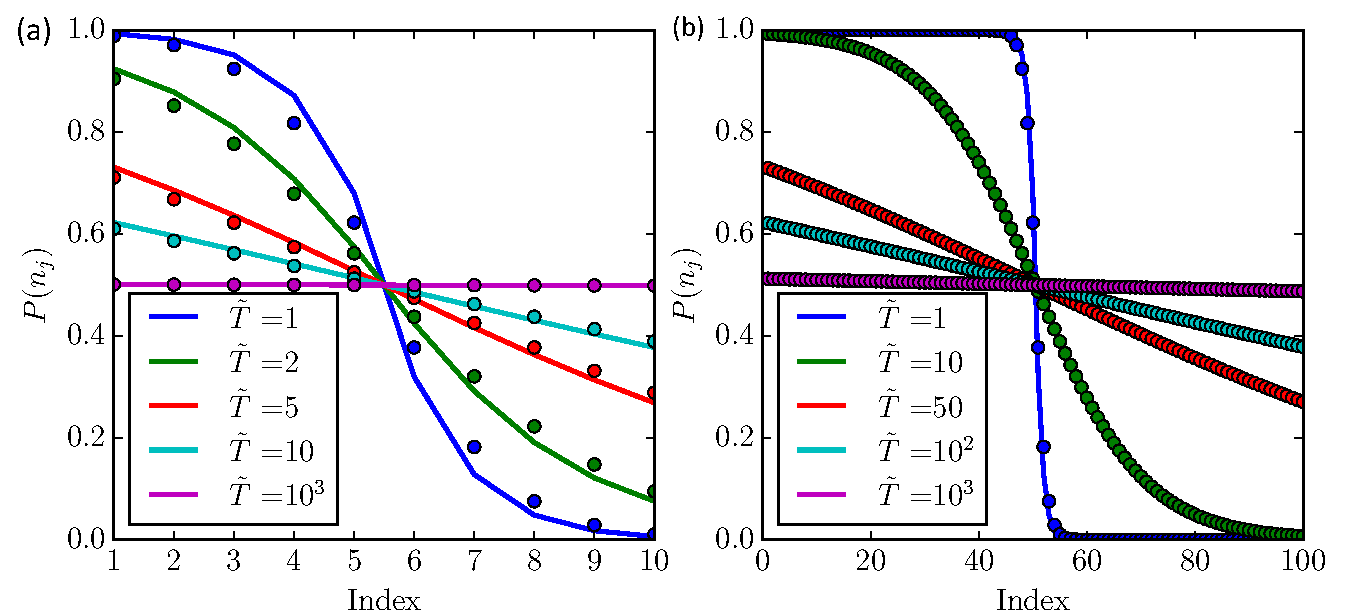
\includegraphics[width=1.0\linewidth]{fermiDirac}
    \caption{Fermi-Dirac distribution compared with the exact solution from the number partition theory. Solid lines are the exact solution while the dots are Fermi-Dirac approximations. Different dimensionless temperature is indicated by different colors as shown in the legend. (a) $L=10$, (b) $L=100$. }
    \label{fig:fermiDirac}
\end{figure}

With Eq. \eqref{eq:fermiDirac}, the mean and variance of random variable $n_j$ can be calculated straightforwardly:
\begin{subequations}
    \begin{align}
        \label{eq:nmean}
        \left<n_j\right> & = \mathbb{P}\left\{n_j=1\right\},\\
        \label{eq:nvar}
        \text{var}\left[n_j\right] & = \mathbb{P}\left\{n_j=1\right\} \cdot \mathbb{P}\left\{ n_j=0\right\} 
        - \left<n_j\right>^2.
    \end{align}
\end{subequations}
On the other hand, from Eq. \eqref{eq:beadposRodsum} and Eq. \eqref{eq:variableu2n} we can calculate the position of bead as
\begin{equation}
    \label{eq:beadpos1D}
    z_i = a\left(2\sum_{j=1}^i n_j - i\right).
\end{equation}
If we assume $n_1, n_2, \cdots, n_L$ are all mutually independent, then the mean and variance of bead position can simply calculated as
\begin{subequations}
    \label{eq:meanVarPos1D}
    \begin{align}
    \label{eq:meanPos1D}
        \left<z_j\right> & = a \left(2\sum_{j=1}^i \left<n_j\right> - i\right),\\
    \label{eq:varPos1D}
        \text{var}\left[z_j\right] & = 4a^2\sum_{j=1}^i\text{var}\left[n_j\right]
    \end{align}
\end{subequations}
The results of the above equations can be compared to the Monte-Carlo simulation (see Appendix \ref{append:mc1D} for details). 
We found that the formula for mean bead position works perfect. However, the formula for variance does not work so good. Notice that Eq. \eqref{eq:varPos1D} is monotonically increasing with the index $i$. We can take the simple symmetric argument that the $\text{var}\left[z_i\right] = \text{var}\left[z_{L-i}\right]$. The result after that still can not match with the simulations. See in Fig. \ref{fig:meanVarAdd1D}.

\begin{figure}[htpb]
    \centering
    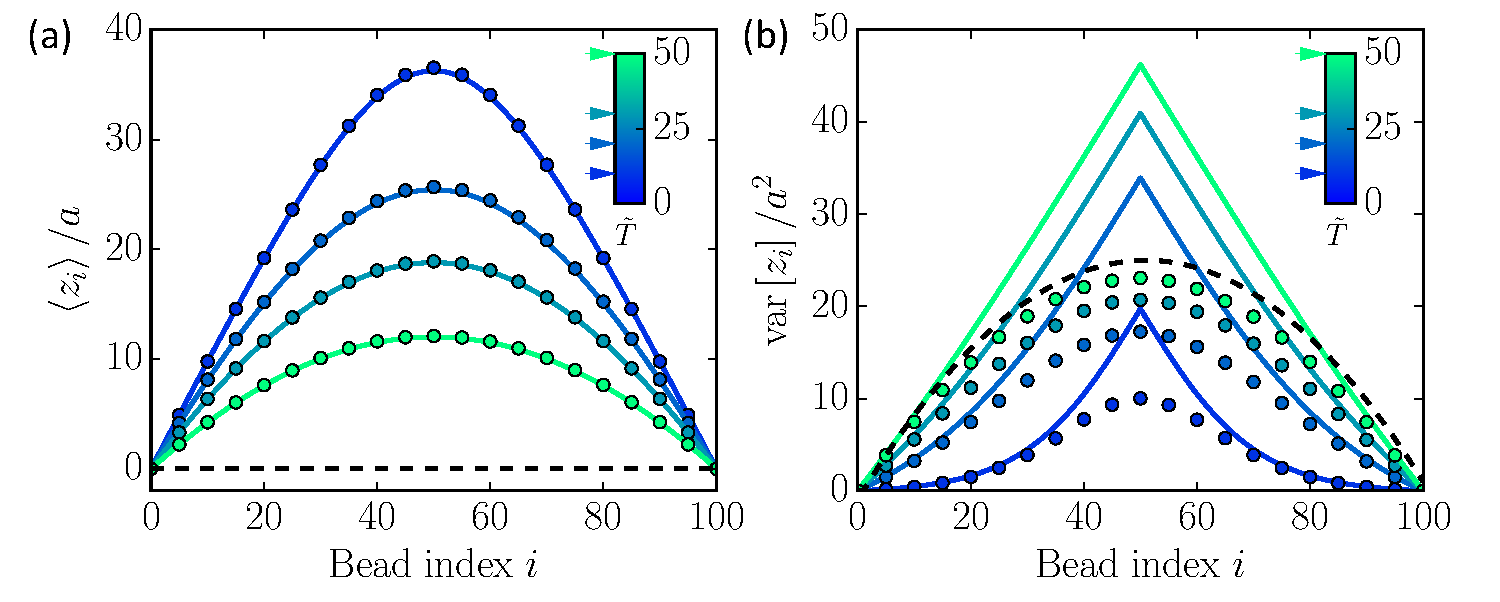
\includegraphics[width=1.0\linewidth]{meanVarAdd1D}
    \caption{Mean and variance of the 1D pinned polymer bead positions. MC simulation results (dots) are compared with theoretical results (solid lines) Eq. \ref{eq:meanVarPos1D}. The length of the polymer loop $L=10$. The black dash line indicates the case $\tilde{T}\rightarrow\infty$, i.e. no external force field. }
    \label{fig:meanVarAdd1D}
\end{figure}

The reason for this mismatch is simple, the particles are not exactly independent and the loop condition is only fulfilled on average by choosing the chemical potential $\mu=(L+1)/2$ in Eq. \eqref{eq:fermiDirac}. In the following part, we will show how to solve this problem use the Brownian bridge technique. 

\subsubsection{The Brownian bridge condition}
\label{ssub:The Brownian Bridge Condition}
Let us consider the polymer loop as a random walk that returns to the origin point after $L$ steps. This sort of random walk process is called the Brownian bridge \cite{Feller2008,Athreya2006}. So each rod represents a random walk step. The segment connecting the $k^{\rm{th}}$ and the $l^{\rm{th}}$ bead corresponds to the propagator $\rho(z_l = z | z_k=0)$. According to the Lindeberg-Feller central limit theorem \cite{Feller2008}, this propagator is Gaussian with the mean and variance equal to the sum of the mean and variance of all individual steps from $k$ to $l$.

As we said above, the grand canonical ensemble only ensures the loop condition on average. To solve the problem, we now impose the Brownian bridge condition so that every single trajectory fulfills the loop condition. The Brownian bridge can be formulated as following:
\begin{equation}
    \label{eq:brownianBridge}
    \rho^L(z_i=z) = \frac{\rho(z_i=z|z_0=0)\rho(z_{L-i}=z|z_L=0)}{\rho(z_L=0|z_0=0)},
\end{equation}
where $\rho(z_i=z)$ is the probability density function of finding the $i^{\rm{th}}$ bead at position $z$, $\rho(z_k=z|z_j=0)$ are the propagators. Eq. \eqref{eq:brownianforce} means that the probability density equals two pieces of random walk trajectory of length $i$ and $L-i$ meet at position $z$ on the condition that they are belong to the same loop. 
\begin{figure}[htpb]
    \centering
    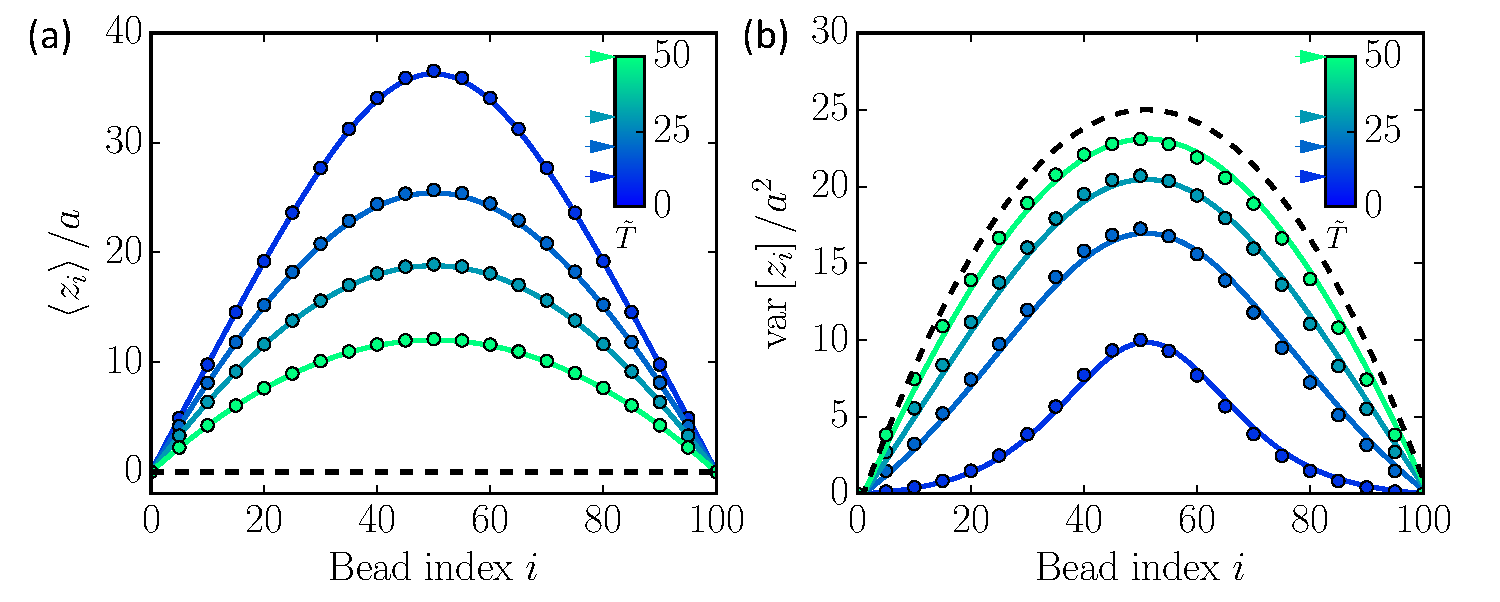
\includegraphics[width=1.0\linewidth]{meanVar1D}
    \caption{Mean and variance of the 1D pinned polymer bead positions. MC simulation results (dots) are compared with theoretical results (solid lines) Eq. \ref{eq:meanVarPos1DExpression}. The length of the polymer loop $L=10$. The black dash line indicates the case $\tilde{T}\rightarrow\infty$, i.e. no external force field. }
    \label{fig:meanVar1D}
\end{figure}

Notice that the propagators are Gaussian with the variance added up by the variance of individual steps, i.e Eq. \eqref{eq:varPos1D}. So that $\rho^L(z_i = z)$ is also Gaussian. Its variance is given by
\begin{equation}
    \label{eq:varBrownianBridge}
    \text{var}\left[z_i\right] = 4a^2\frac{\sum_{j=0}^{i}\text{var}\left[n_j\right]\sum_{j=L-i}^{L}\text{var}\left[n_j\right]}{\sum_{j=0}^{L}\text{var}\left[n_j\right]}.
\end{equation}
Plug in Eq. \eqref{eq:nvar} and Eq. \eqref{eq:varPos1D} we can obtain the variance of bead position in the loop. For $\tilde{T}\gg 1$, we can obtain the close form expressions for mean and variance of bead position by converting the summation to integral
\begin{subequations}
    \label{eq:meanVarPos1DExpression}
    \begin{align}
        \left< z_i \right> & = 2 a \tilde{T} \ln\left[ \frac{1+\exp\left(\frac{L}{2\tilde{T}}\right)}{\exp\left(\frac{i}{2\tilde{T}}\right) + \exp\left(\frac{L-i}{2\tilde{T}}\right)} \right] \\
        \text{var}\left[z_i\right] & = 2 a^2 \tilde{T} \frac{ \sinh\left( \frac{L-i}{2\tilde{T}}\right) \sinh\left( \frac{i}{2\tilde{T}}\right)} {\sinh\left( \frac{L}{2\tilde{T}}\right) \cosh^2\left( \frac{L-2i}{4\tilde{T}}\right)}
    \end{align}
\end{subequations}
We can see from the above formulas that the $z_i-z_{L-i}$ symmetry is satisfied. And a strong external force field leads to a stretched configuration and a small fluctuation of bead position. This result is compared with the Monte-Carlo simulations, see in Fig. \ref{fig:meanVar1D}.

In this subsection, we solved the mean and variance of bead position for 1D pinned polymer loop in an external force field. The strategy is using the \emph{Fermi-Dirac} statistics and re-enforce the loop condition by the Brownian bridge technique. Excellent results verified by the Monte-Carlo simulation are obtained. However, we have to say, this is just an approximate method. In the next subsection, we will use the canonical ensemble to obtain the exact solution. 

\subsection{Canonical ensemble solution}
\label{sub:canonical_ensemble_solution}
In the particle-lattice picture, the system is actually a canonical ensemble system because of the conservation of particle number. In this section, we will calculate the exact partition function using this ensemble. More interestingly, we will show the calculation can be recoded to a number partition problem. Exact results are obtained and compared with the results from the approximate approach above.

\subsubsection{The number partition theory}
\label{ssub:The Number Partition Theory}
Before the calculation of exact partition function, let us discuss an interesting number partition problem that share a lot of similarities with the former. 

Consider a non-negative integer number $K$, which can be expressed into the summation of $N$ non-negative integers:
\begin{equation}
    K = \sum_{j=1}^N k_j
\end{equation}
However, there is a constraint on the summation components $0 \leqslant k_1 \leqslant k_2 \cdots \leqslant k_N \leqslant M$. This kind of problem can be best visualized by what called Young diagram \cite{Andrews1998}, shown in Fig. \ref{fig:young}.
\begin{figure}[htpb]
    \centering
    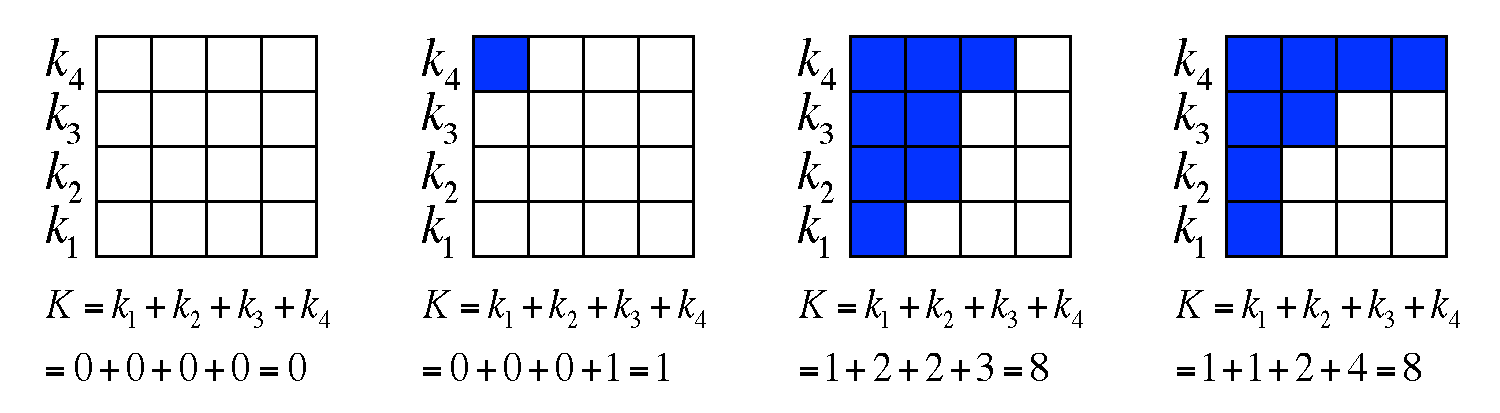
\includegraphics[width=1.0\linewidth]{young}
    \caption{Some examples of the Young diagram.}
    \label{fig:young}
\end{figure}
In the Young diagram, each row represents a integer number. The number of blue boxes means the value of the $j^{\rm{th}}$ integer. Starting from the bottom, because of the constraint, the diagram is non-decreasing. 

The question is, given a certain integer $K$, how many different ways are there to partition it into $N$ non-decreasing pieces $\{k_1, k_2, \cdots, k_N\}$. For the simple cases, one can tell the answer immediately. For examples, in the first two examples of Fig. \ref{fig:young}, we illustrate that there are only one way to partition integer $0$ or $1$ into $4$ non-decreasing integers. However, this question in the general case is not intuitive. Fortunately, this problem is well studied by mathematicians. Let $g(M, N; K)$ denote the number of partitions of $K$ with at most $N$ parts, each of size at most $M$. Equivalently, these are the partitions whose Young diagram fits inside an $N \times M$ rectangle. Then we have the following generating function:
\begin{equation}
    \label{eq:generatingDegeneracy}
    \Phi(q):=\sum_{K=0}^{MN} g(M, N; K) q^K = \binom{M+N}{N}_q
\end{equation}
where $q$ is an auxiliary number, and the notation at the right hand side of Eq. \eqref{eq:generatingDegeneracy} is called $q$ binomial coefficient or Gaussian binomial coefficient. It is defined as 
\begin{equation}
    \label{eq:qBinomial}
    \binom{L}{N}_q := \frac{[L]_q!}{[L-N]_q![N]_q!},
\end{equation}
and $[N]_q := 1 + q + q^2 + \cdots + q^{N-1}$ is called a $q$ number \cite{Andrews1998}.


\subsubsection{Exact partition function}
\label{ssub:Exact Partition Function}
Now, let us start to calculate the partition function of our pinned polymer in the particle-lattice picture. The partition function of a canonical ensemble system with discrete energy can be written as:
\begin{equation}
    \label{eq:partitionFuncCanonical}
    \mathcal{Z}\left(T\right) = \sum_{E}g(E)\exp \left(-\frac{E}{k_B T}\right),
\end{equation}
where $g(E)$ is the degeneracy of the microscopic states which have the same energy $E$. Once $g(E)$ is known, the partition function can be calculated straightforwardly.

Let us take a look at the energy of the system, i.e. Eq. \eqref{eq:energy1DRewrite}. It is represented in the way of rod orientation $u_j$ or occupation variable $n_j$. Here, we are going to use another way to represent the energy. In the particle-lattice picture, the system consists $N:=L/2$ particles. So the energy can be rewritten as:
\begin{equation}
    E = \tilde{E}_0 + \sum_{j=1}^N E_j,
\end{equation}
where $E_j$ is the energy of the $j^{\rm{th}}$ particle in the external force field. Again, $\tilde{E}_0$ is an unimportant constant energy offset. Denote the position of the $j^{\rm{th}}$ particle as $x_j$, which is an integer $x_j\in[1, L]$. Then we can write $E_j = x_j \Delta E$. 
Also notice that, because of the exclusive condition, the sample space of the particle system is constrained in $\Omega = \{\mathbf{x}| 1\leqslant x_1<x_2<\cdots<x_N\leqslant L\}$.

Let us do a shift for the particle position by defining
\begin{equation}
    k_j := x_j - j.
\end{equation}
Notice now the constraint on $x_j$ is transferred to $0 \leqslant k_1 \leqslant k_2 \cdots \leqslant k_N \leqslant N$. And the energy of the system can be rewritten as:
\begin{equation}
    E = \hat{E}_0 + \Delta E \sum_{j=1}^N k_j = \hat{E}_0 + K \Delta E,
\end{equation}
Again $\hat{E}_0$ here is an unimportant constant energy offset, $\hat{E}_0 = \tilde{E}_0+N(N+1)/2$. 
It is not difficult to find the range of the energy is $\hat{E}_0, \hat{E}_0 + \Delta E, \cdots, \hat{E}+N^2\Delta E$. 

Now we are closer to the number partition problem. Notice that $K=\sum_{j=1}^{N}k_j$ and we have the same type of constraint as in the number partition problem. In addition, because the mapping from integer $K$ to energy $E$ is one-to-one. So the degeneracy function $g(E)$ is exactly the number of ways to partition the integer $K$. Furthermore, let us denote $q:=\exp\left(-\Delta E/ k_B T\right)$. Then we have
\begin{equation}
    \begin{aligned}
    \label{eq:partitionFuncExact}
    \mathcal{Z}\left(T\right) & = \sum_{E}g(E)\exp \left(-\frac{E}{k_B T}\right) \\ 
    & = \exp\left(-\frac{\hat{E}_0}{k_B T}\right)\sum_{K=0}^{N \times N} g(N, N; K) q^K \\
    & = \exp\left(-\frac{\hat{E}_0}{k_B T}\right)\binom{L}{N}_q.
    \end{aligned}
\end{equation}


With the exact partition function Eq. \eqref{eq:partitionFuncExact}, the equilibrium distribution can be calculated straightforwardly:
\begin{equation}
    \label{eq:equilibriumDistr}
    P^{e} = \frac{1}{\mathcal{Z}\left(T\right)}\exp\left(-\frac{E}{k_B T}\right) = \frac{q^K}{\binom{L}{N}_q}.
\end{equation}
We can see here the offset energy is not in the distribution function. That is why we always say it is not important. In principle, Eq. \eqref{eq:equilibriumDistr} is not an exact relation. It might still have a constant pre-factor which can be fixed by the normalization condition $\sum_{K=0}^{N^2} P^e = 1$. However, the constant is not important for our discussions, so we will just keep it in the form of Eq. \eqref{eq:equilibriumDistr}.

With Eq. \eqref{eq:partitionFuncExact} and Eq. \eqref{eq:equilibriumDistr}, in principle, one can calculate whatever equilibrium quantities. Here, we will calculate the probability distribution of rod orientation in order to compare with our previous approach based on grand canonical ensemble. 

\subsubsection{Exact probability distribution of the rod orientation}
\label{ssub:Exact probability distribution of the rod orientation}
The probability distribution of rod orientation is equivalent to the probability distribution of the lattice site occupation. Previously, we have employed the \emph{Fermi-Dirac} distribution. In this subsection, we will calculate the exact distribution of $\mathbb{P}\{n_j=1\}$ to show how accurate the \emph{Fermi-Dirac} distribution is. 

In order to do that, let us first rewrite the equilibrium distribution Eq. \eqref{eq:equilibriumDistr} in the coordinate of particle position:
\begin{equation}
    \label{eq:equilibriumDistrPos}
    P^e(x_1, x_2, \cdots, x_N) = q^{-\frac{N(N+1)}{2}} {\binom{L}{N}_q}^{-1}\prod_{i=1}^N q^{x_i}.
\end{equation}

Now let us denote $P_i(x)$ the probability that the $i^{\rm{th}}$ particle is at position $x$. Then $P_i(x)$ can be calculated as 
\begin{equation}
    \begin{aligned}
        \label{eq:pdfTaggedParticle}
        P_i(x) = & \sum_{1 \leqslant x_1<\cdots<x_{i-1}\leqslant x-1}P^e(x_1, x_2, \cdots, x_N) \\
        &\times \sum_{x<x_{i+1}<\cdots<x_{N}\leqslant L}P^e(x_1, x_2, \cdots, x_N) \\
        = & \left. q^{(N+1-i)(x-i)} \binom{x-1}{i-1}_q\binom{L-x}{N-i}_q 
            \middle/  \binom{L}{N}_q \right..
    \end{aligned}
\end{equation}

Finally, the probability that the $j^{\rm{th}}$ sites is occupied can be calculated as
\begin{equation}
    \label{eq:exactOccupationProb}
    \mathbb{P}\{n_j=1\} = \sum_{i=1}^N P_i(x=j) 
\end{equation}
Eq. \eqref{eq:exactOccupationProb} simply means the probability of one site is occupied is the sum of the probability that it is occupied by any particles. Plug in Eq. \eqref{eq:pdfTaggedParticle}, one can obtain the exact occupation probability distribution. This is compared with the \emph{Fermi-Dirac} distribution in Fig. \ref{fig:fermiDirac}. As we can see in the figure, the discrepancy is quite small. It is only noticeable for a small lattice size at very strong external force field, see in Fig. \ref{fig:fermiDirac} (a). So the Fermi-Dirac distribution is actually a very accurate approximation. 


In this section, we solve the equilibrium statistics of the pinned polymer loop model in 1D. Utilizing the mapping from the polymer to a particle-lattice system, we solve the statistics by two different approaches. The first one employs the famous \emph{Fermi-Dirac} distribution and the Brownian bridge technique. However, it is an approximate method. The second method based canonical ensemble and number partition theory is an exact solution. The exact results are compared with the first methods as well as the Monte-Carlo simulations. Our theory matches very well to the simulation results. In next section, we will extend our theory to the 3D system. 




%********************************** % Third Section  *************************************
\section{Equilibrium statistics in 3D}
\label{sec:equilibrium_statistics_in_3d}
In 3D, the equilibrium statistics of the pinned polymer loop model can still be calculated using the similar strategy. The orientation of rods have two more degree of freedom in 3D. As shown in section \ref{sec:pinned_polymer_loop}, the external force is assume in the $z$ direction. Let us use the spherical coordinates to describe the polymer system. Denote $\theta_j$ the angle between the $j^{\rm{th}}$ rod and the $z$-axis, and $\phi_j$ the rotational angle along $z$-axis. Then the loop condition along the force direction can be written as
\begin{equation}
    \label{eq:loopCondition3D}
    \sum_{j=1}^L \cos\theta_j = 0.
\end{equation}
Using the above condition, the energy of the 3D polymer Eq. \eqref{eq:energyRodsum} can be rewritten as 
\begin{equation}
    \label{eq:energy3D}
    E = E_0 + Fa\sum_{j=1}^L j\cos\theta_j.
\end{equation}

In the following subsections, we will first derive the partition function, and then calculate the mean and variance of the three dimensional beads position. 

\subsection{Partition function}
\label{sub:partition_function}
To calculate the equilibrium statistics of 3D bead-rod system, we will use the approach of grand canonical ensemble combined with the Brownian bridge condition. The grand canonical ensemble partition function can be written as:
\begin{equation}
    \label{eq:partitionFunc3D}
    \mathcal{Z} = \prod_{j=1}^L \mathcal{Z}_j = \prod_{j=1}^L \int_{0}^{2\pi} d\phi \int_{0}^{\pi}\exp\left(-\frac{(j-\mu)\cos\theta\Delta E}{k_BT}\right).
\end{equation}
Here, $\mu=(L+1)/2$ is the chemical potential the same as in 1D. However, $\Delta E = Fa$ is different from the 1D case. Again, let us define the \emph{dimensionless temperature}:
\begin{equation}
    \tilde{T} = \frac{k_B T}{\Delta E} = \frac{k_B T}{Fa}.
\end{equation}
There is a factor of two compare to the dimensionless temperature in 1D.

The integration can be calculated in Eq. \eqref{eq:partitionFunc3D}, which turns out
\begin{equation}
    \label{eq:partitionFuncRod}
    \mathcal{Z}_j = \frac{\tilde{T}\sinh\frac{j-\mu}{\tilde{T}}}{j - \mu}.
\end{equation}
So the mean and variance of the $j^{\rm{th}}$ rod orientation $u_{j,z} = \cos\theta_j$ can be calculated as
\begin{equation}
    \begin{aligned}
    \label{eq:meanVarRod}
    \left<\cos\theta_j\right> = \tilde{T}\partial_{\mu}\ln\mathcal{Z}_j = \coth\frac{\mu - j}{\tilde{T}}-\frac{\tilde{T}}{\mu-j}, \\
    \text{var}\left[\cos\theta_j\right] = \tilde{T}^2\partial_{\mu}^2\ln\mathcal{Z}_j = \frac{\tilde{T}^2}{(j-\mu)^2} - \text{csch}^2\frac{j-\mu}{\tilde{T}}.
    \end{aligned}
\end{equation}
Notice that, for symmetry reasons, the average projection for $x$ and $y$ directions are zero: $\left<u_{j,x}\right> = \left<u_{j,y}\right> = 0$. The second moment of these component can be calculated as
\begin{equation}
    \label{eq:second_moment}
    \left<u_{j,x}^2\right> = \left<u_{j,y}^2\right> = (1-\left<\cos^2\theta_j\right>)/2
\end{equation}

The above equations give the statistical properties of individual rod orientation. In next subsection, we will use the Brownian bridge technique to calculate the mean and variance of beads position.

\subsection{Mean and variance of the bead position}
\label{sub:mean_and_variance_of_bead_position}
In the case of 3D pinned polymer, according to Lindeberg-Feller central limit theorem \cite{Feller2008,Athreya2006}, the corresponding random walk is a multi-variate Gaussian process. It can be factorized into the product of three Gaussian processes, each corresponding to a coordinate axis. Let us first discuss it in the $z$ direction, i.e. the direction along the force field. The propagator in the $z$ direction $\rho(z_k = z| z_0 = 0)$ is Gaussian with the following mean and variance:
\begin{equation}
    \begin{aligned}
    \label{eq:meanVarRod3D}
    \left<z_k\right> = a\sum_{j=1}^k\left<\cos\theta_j\right>, \\
    \sigma_{0 \rightarrow k,z}^2 = a^2\sum_{j=1}^k\text{var}\left[\cos\theta_j\right].
    \end{aligned}
\end{equation}

Finally, by imposing the Brownian bridge condition, the variance of bead position can be written as 
\begin{equation}
    \label{eq:varBrownianBridge3D}
    \text{var}\left[z_k\right] = a^2\frac{\sum_{j=0}^{k}\text{var}\left[\cos\theta_j\right]\sum_{j=L-k}^{L}\text{var}\left[\cos\theta_j\right]}{\sum_{j=0}^{L}\text{var}\left[\cos\theta_j\right]}.
\end{equation}
The analytical results above are compared with the 3D Monte-Carlo simulations (see section \ref{sec:monte_carlo_simulation_of_the_bead_rod_model}). We can see in Fig. \ref{fig:meanVarZ3D} that again an excellent agreement is obtained. 

\begin{figure}[htpb]
    \centering
    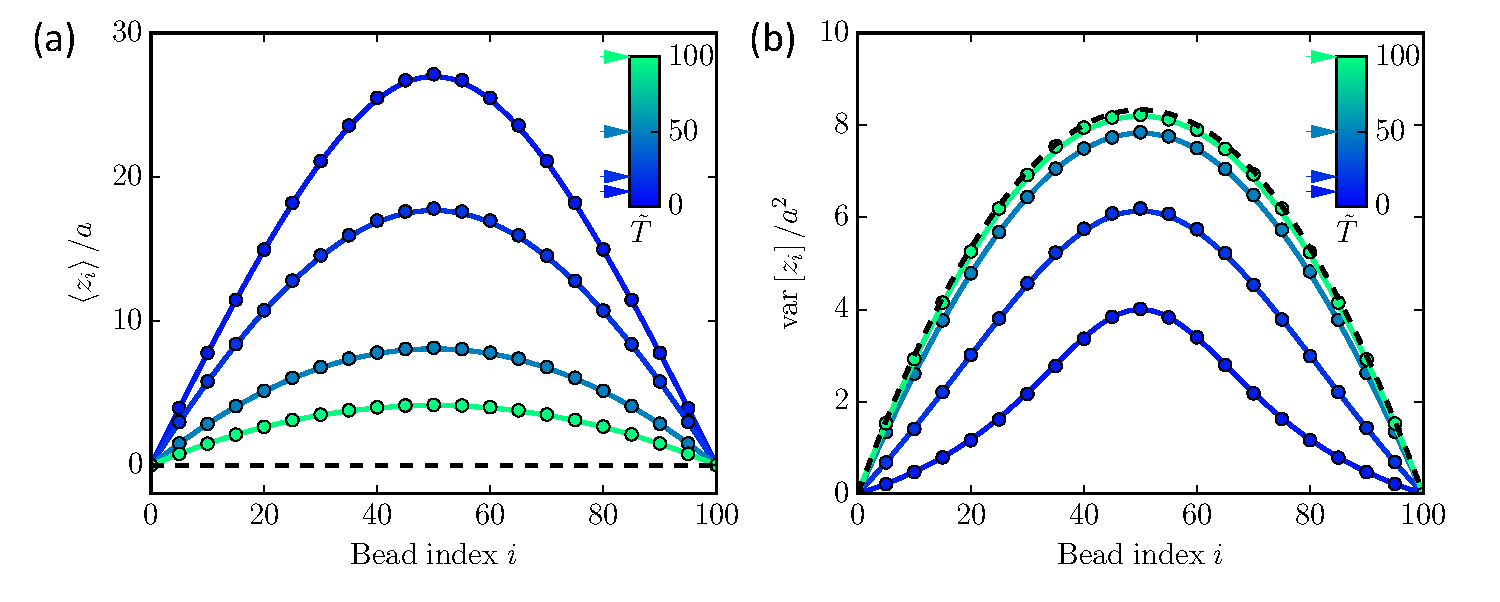
\includegraphics[width=1.0\linewidth]{meanVarZ3D}
    \caption{Mean and variance of the bead position in the direction along the force field. Solid lines are theory and dots are Monte-Carlo simulation results. The black dash line indicates the case $\tilde{T}\rightarrow\infty$, i.e. no external force field.}
    \label{fig:meanVarZ3D}
\end{figure}

Now let us discuss the directions perpendicular to the force direction. By symmetric reasons, we can immediately conclude that the statistics in $x$ and $y$ directions are identical. In addition, the mean position in both direction should be vanished because there is no bias. We can write as
\begin{equation}
    \label{eq:xyMean}
    \left<x_k\right> = \left<y_k\right> = 0.
\end{equation}

On the other hand, using Eq. \eqref{eq:second_moment}, the variance of $x$ and $y$ components of the $j^{\rm{th}}$ rod orientation can be written as
\begin{equation}
    \label{eq:xyRodVar}
    \text{var}\left[u_{j,x}\right] = \text{var}\left[u_{j,y}\right] = \left<u_{j,x}^2\right> - \left<u_{j,x}\right>^2 = (1-\left<\cos^2\theta_j\right>)/2
\end{equation}
Again, impose the Brownian bridge condition similar to Eq. \eqref{eq:varBrownianBridge3D}, the variance of $x$ and $y$ components of the bead position can be obtained. Notice the variance in $x$ and $y$ directions are different from the variance in $z$ direction. This is shown in Fig \ref{fig:xyVar3D} together with the benchmark of our theory and the Monte-Carlo simulations.

\begin{figure}[htpb]
    \centering
    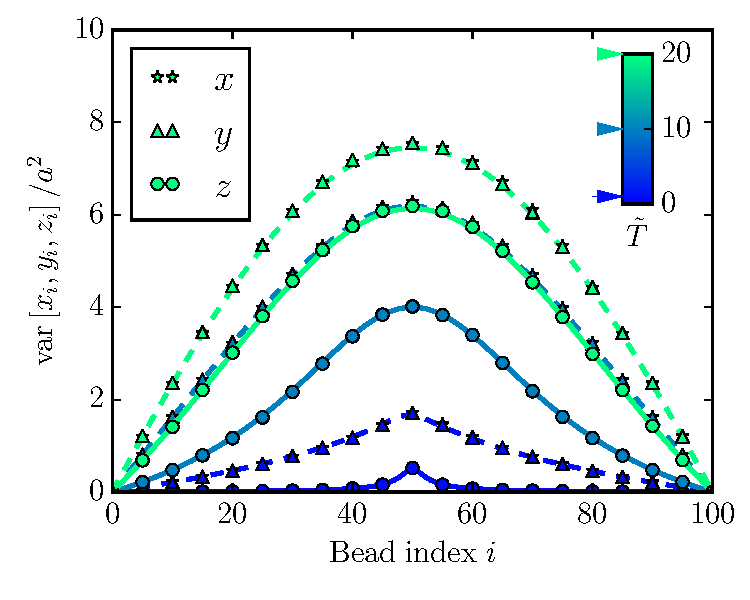
\includegraphics[width=0.6\linewidth]{xyVar3D}
    \caption{Comparison of fluctuations in $x$, $y$ and $z$ directions. Symbols denote the Monte-Carlo simulations. Circles show the fluctuations along the $z$ axis, whereas stars and triangles along $x$ and $y$ axis respectively. Colors correspond to different dimensionless temperatures. Solid and dashed lines are theoretical predictions for fluctuations along and orthogonal to the force field, respectively.}
    \label{fig:xyVar3D}
\end{figure}


\subsection{The pairing of loops and intersecting loops}
\label{sub:the_pairing_of_loops_and_intersecting_loops}

In fission yeast, the chromosomes are appearing in pairs during nuclear oscillation, which means there are two mechanically identical chromosomes. And there are three chromosome pairs in fission yeast in total. The biological facts motivate us to consider a pair of polymer loops pinned at the same point. 
Biologically, recombination happens during nuclear oscillation. It is essential for homologous to come close spatially in order to recombine, which is done by a paring process. Thus it is meaningful to study to statistical distance between two corresponding loci along the polymer loops.
Physically, the pairing process of homologous is often said to be analogy to the zipping process of a zipper~\cite{Tsai2011}. Namely, segments near to the SPB are paired in prior. However, biologists suspect some additional connections between homologous could have been formed before the paring. And one of the hypothesises is that the centromeres of homologous are still bond together during nuclear oscillation. So these facts motivate us to consider the intersecting polymer loops with the same pinned point. In this subsection, we will calculate these cases in the 3D settings.

Firstly, let us discuss the paring of two identical polymer loops pinned at the same point. Fig. \ref{fig:pair} is the schematic of this case.
\begin{figure}[htpb]
    \centering
    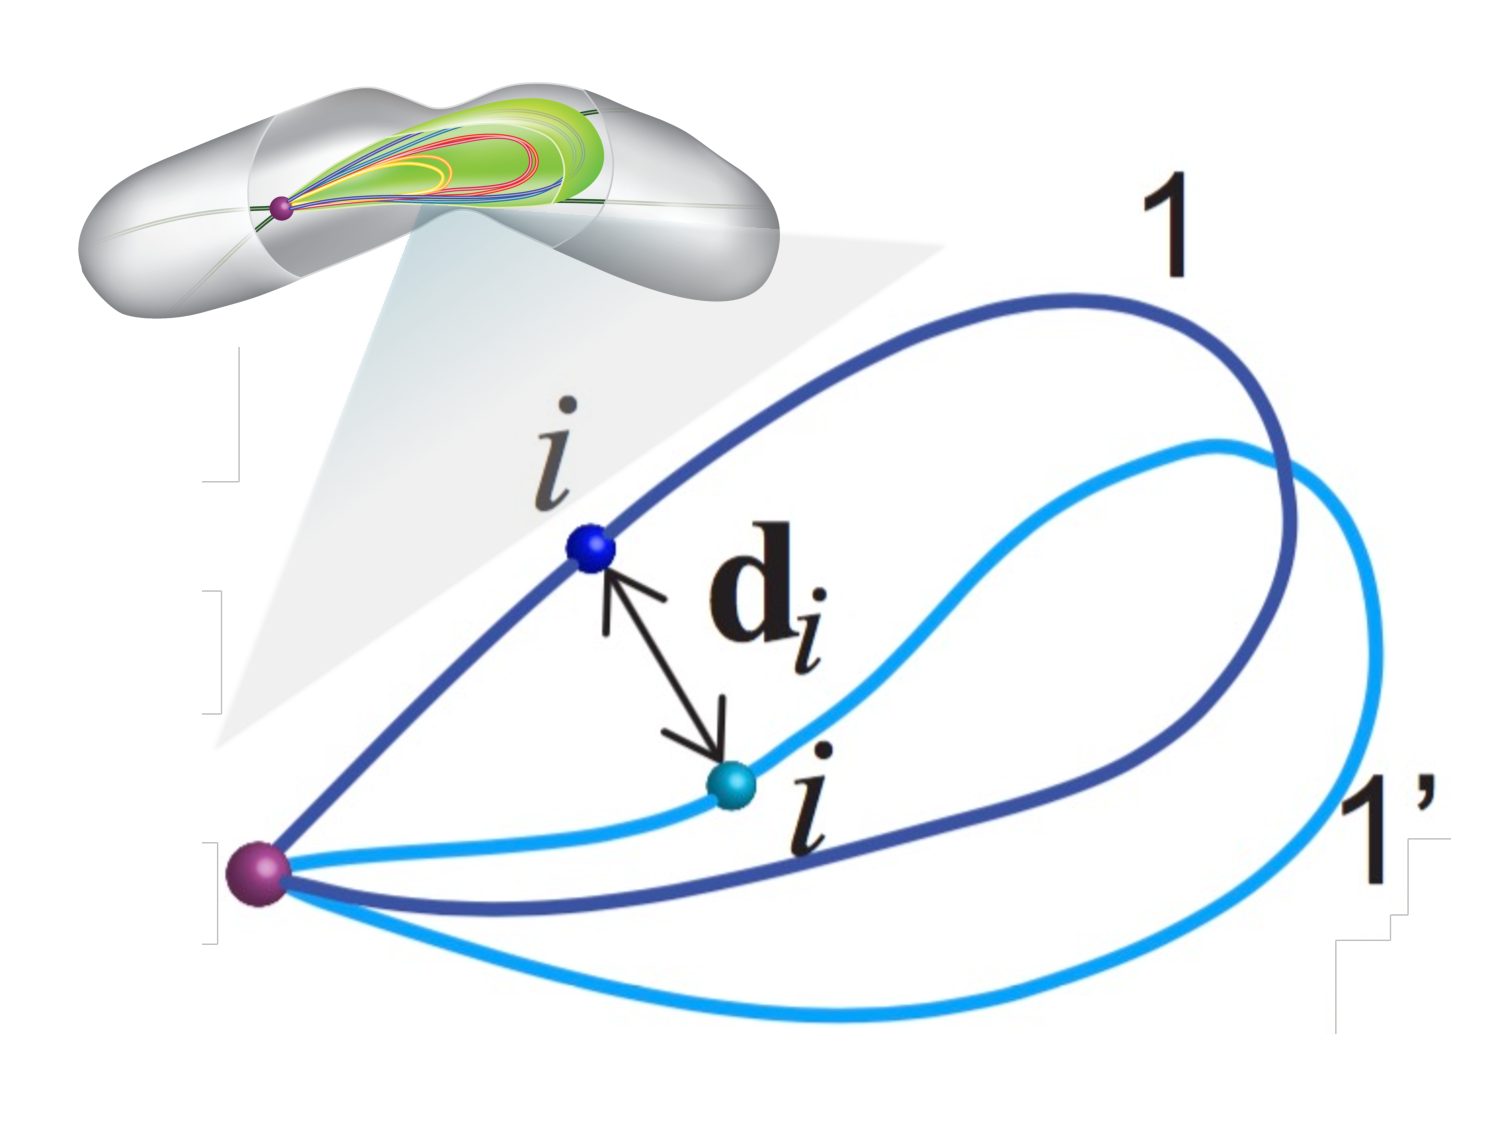
\includegraphics[width=0.6\linewidth]{pairLoops}
    \caption{A Pair of polymer loops pinned at the same point representing the homologous. The distance of a pair of loci is illustrated as $\mathbf{d}_i$. }
    \label{fig:pairLoops}
\end{figure}

Given that the excluded volume effect is ignored, the three dimensional mean distance between two corresponding beads is zero. The statistical distance is defined as the square root of its variance and the variance is calculated as:
\begin{equation}
    \label{eq:statisticalDistance}
    \text{var}\left[\mathbf{d}_i\right] = 
    \text{var}\left[\mathbf{r}_i - \mathbf{r}_i^\prime\right] = 2 \text{var}\left[\mathbf{r}_i\right]
    = 2\left( \text{var}\left[x\right] + \text{var}\left[y\right] + \text{var}\left[z\right]\right).
\end{equation}
In Fig.~\ref{fig:pairing} we show the statistical distance varies with the dimensionless temperature, which is the inverse measure of the external force field strength.
We can see from the figure that strong force field reduces the statistical distance thus facilitates pairing. BD simulations are performed and results are found match to our theory. 
\begin{figure}[htpb]
    \centering
    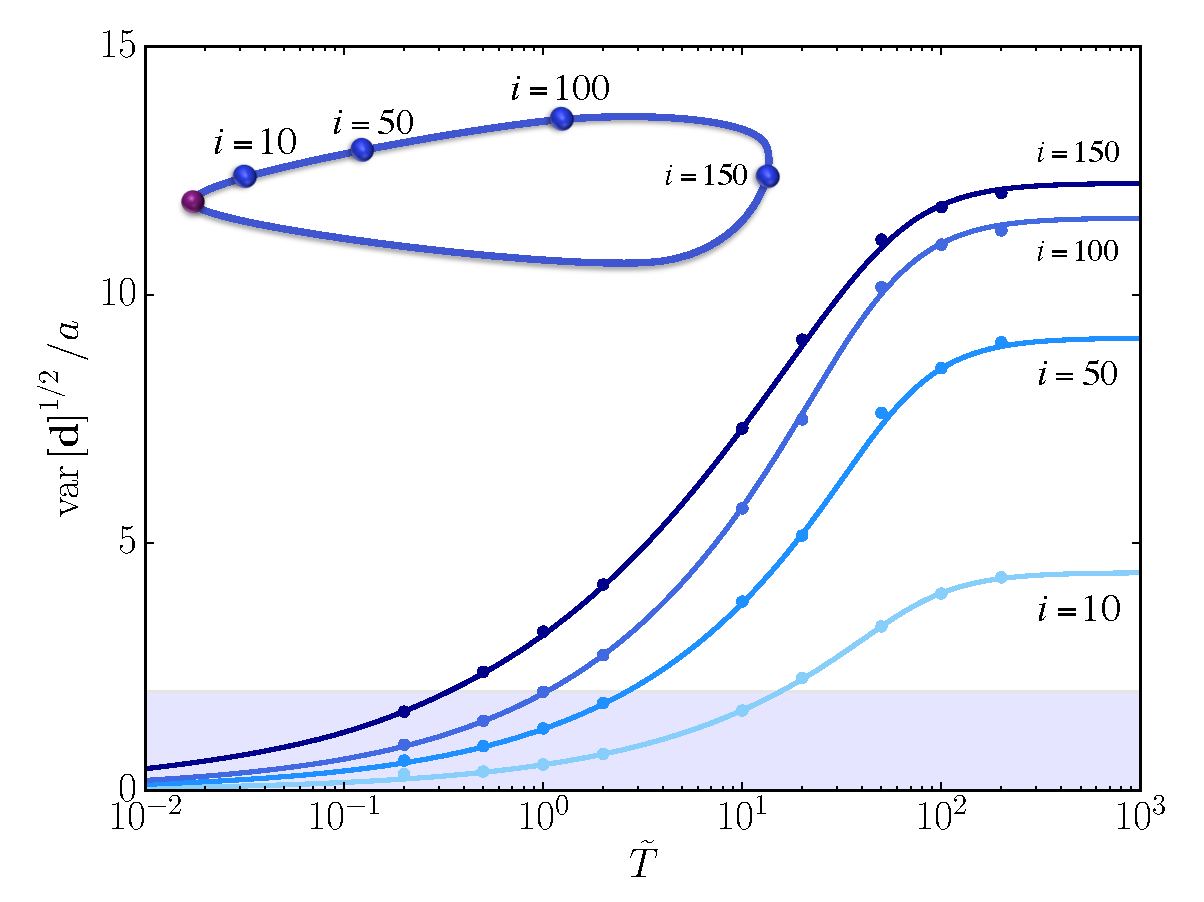
\includegraphics[width=0.7\linewidth]{pairing}
    \caption{The distance between corresponding loci of polymer pair loops varies withe the dimensionless temperature. Different curve indicates different location along loop. The shaded region the paired distance. Dots are BD simulation data and solid lines are results from our theory. Inset is an sketch of the observing loci along the chromosome. $L=300,~k_BT=1$ are set.}
    \label{fig:pairing}
\end{figure}

Now let us discuss the case of pairing with an additional intersecting in the middle of polymer loops. The schematic of this case is shown in Fig.~\ref{fig:centromere}.
\begin{figure}[htpb]
    \centering
    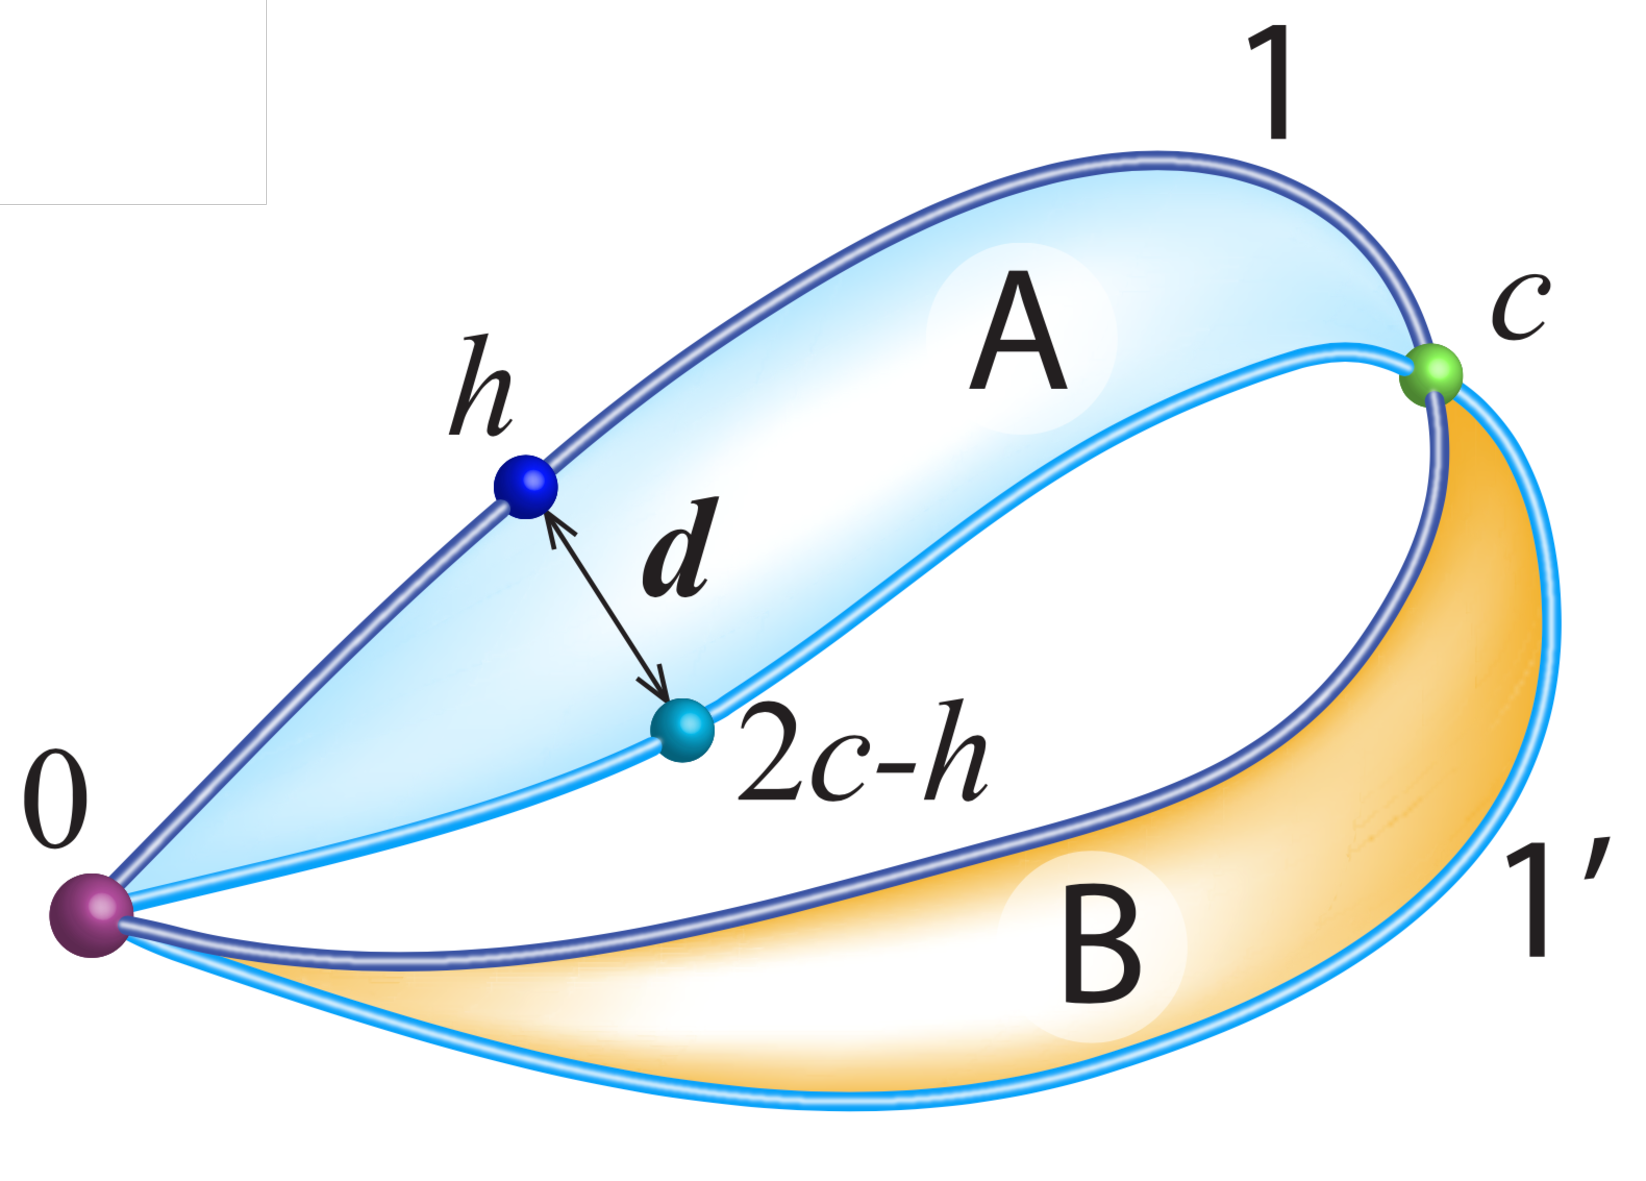
\includegraphics[width=0.6\linewidth]{centromere}
    \caption{The sketch of two intersecting loops $1$ and $1^\prime$ which are connected at one additional bead with index $c$. Shaded regions indicate the redefined loops A and B. The distance $\mathbf{d}$ between two homologous beads $h$ and $2c-h$ is illustrated. }
    \label{fig:centromere}
\end{figure}
The pair of polymer loops (denoted by $1$ and $1^\prime$) pinned at the same point $0$ with an additional constraint at some intermediate bead position (indexed by $c$, where $0<c<L$). However, bead $c$ is not pinned so that it can still move around. 

In order to solve this problem, we redefine the loops as shown in Fig.~\ref{fig:centromere}. The loop A starts at the pinned point, continues along the loop $1$, to the constraint point $c$ and then returns to the origin along the loop $1^\prime$ by the path of the same length. It is shown in Fig.~\ref{fig:centromere} shaded with cyan color in between. The loop B is shown in Fig.~\ref{fig:centromere} shaded with orange color in between. We are interested in the distance $\mathbf{d}$ between two homologous beads as shown in the figure. Denote the first bead position with index $h$, then the other one can be denoted by $2c-h$ considering the loop A. 
\begin{figure}[htpb]
    \centering
    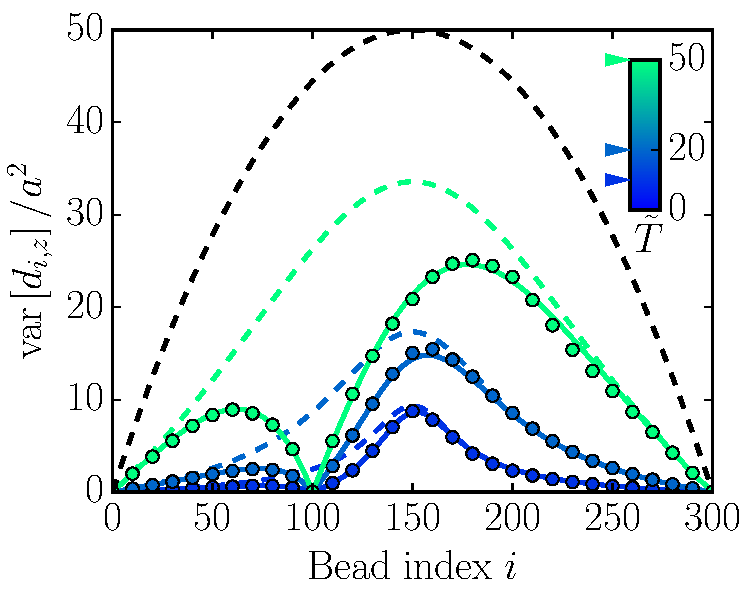
\includegraphics[width=0.6\linewidth]{varCentromere}
    \caption{Variance of the distance between pinned polymer loops with additional constraint. The constraint is located at the bead with index $c=100$. Circles denote the simulation results while the solid lines represent the theory. The dashed lines show the variance of the unconstrained case with different color indicates different dimensionless temperature. The black dashed line shows the limit of unconstrained force-free Brownian bridge.}
    \label{fig:varCentromere}
\end{figure}

To calculate the PDF of $\mathbf{d} := \mathbf{r}_h - \mathbf{r}_{2c-h}$, which denote as $\rho(\mathbf{d})$, let us first calculate the joint positional PDF $\rho_{h, 2c-h}(\mathbf{r}_1, \mathbf{r}_2)$. Denote the propagator as $\rho_{k\rightarrow j}(\mathbf{r}_1 | \mathbf{r}_2) = \rho(\mathbf{r}_k = \mathbf{r}_1 | \mathbf{r}_j = \mathbf{r}_2)$. Notice that the propagator is a (multi-variate) Gaussian function with a mean and variance summing up by path steps. Then we can apply the similar Brownian bridge condition, obtaining
\begin{equation}
    \label{eq:jointPdfDistance}
    \rho_{h,2c-h}(\mathbf{r}_1, \mathbf{r}_2) = \frac{\rho_{0\rightarrow h}(\mathbf{r}_1|0)\rho_{h\rightarrow 2c-h}(\mathbf{r}_1|\mathbf{r}_2)\rho_{0\rightarrow 2c-h}(\mathbf{r}_2|0)}{\rho_{0\rightarrow 2c}(0|0)}.
\end{equation}
And then the PDF $\rho(\mathbf{d})$ can be calculated as 
\begin{equation}
    \label{eq:pdfDistance}
    \rho(\mathbf{d}) = \int\int d\mathbf{r}_1 d\mathbf{r}_2 \delta(\mathbf{d} - (\mathbf{r}_1 - \mathbf{r}_2))\rho_{h, 2c-h}(\mathbf{r}_1, \mathbf{r}_2),
\end{equation}
Without evaluate the integrals in Eq. \eqref{eq:pdfDistance}, one can conclude $\rho(\mathbf{d})$ is Gaussian because $\rho_{h,2c-h}(\mathbf{r}_1, \mathbf{r}_2)$ is Gaussian. It is not difficult to obtain the mean distance is $\left<\mathbf{d}\right>=\mathbf{0}$ because of no excluded volume effect. And the variance can calculate the same way as our previous procedure. For example, the $z$-component variance is
\begin{equation}
    \label{eq:zvarDistance}
    \text{var}\left[ d_z \right] = 2 \frac{\sigma_{0\rightarrow h,z}^2\sigma_{h\rightarrow c,z}^2}{\sigma_{0\rightarrow c,z}^2}, 
\end{equation}
where each variance is calculated according to Eq. \eqref{eq:meanVarRod}. The result compare with simulations is shown in Fig. \ref{fig:varCentromere}. We see that fluctuations of the distance is reduced with the additional constraint point compared with the unconstrained case. 

In this section, we discussed the three dimensional pinned polymer loop model and its equilibrium statistics. The mean and variance of each bead position are calculated using the grand canonical ensemble combined with Brownian bridge technique. 
Fluctuations of distance between corresponding beads of pinned polymer pair loops are calculated analytically to quantify the paring process. The theoretical results are all verified by simulations. In addition, by discussing the case of two intersecting polymer loops, we find the additional constraint helps to reduce the fluctuations, thus facilitate the pairing process. 
In next section, we will use the theory of equilibrium statistics to quantify the shape of polymer loops in an external force field.


%********************************** % Fourth Section  *************************************
\section{Characterizing the shape of pinned polymer loops}
\label{sec:characterizing_the_shape_of_pinned_polymer_loops}

We have shown the in Fig. \ref{fig:oscillation} the stained chromosomes during nuclear oscillation. Experimentally, it is relatively easier to measure the shape of the chromosomes. 
On the other hand, the shape of the chromosomes is believed to be important for the paring process of homologous. For example, it is reported in \cite{Chacon2016} that the expression of the LinE protein Rec25 is promoted in elongated nucleus than the round shaped nucleus. So it is meaningful to characterize the shape of the chromosomes quantitatively. 

In this section, we will introduce several indicators used to quantify the shape of steady state chromosomes, which is modeled by the pinned polymer loops. We will introduce the three dimensional gyration tensor, asphericity and the nature of asphericity. The simulation results are compared with the theory from preceded sections. We will also try to compare our theory to the blob theory, which is known as the ``stem-flower'' shape of pinned polymer chain. 


\subsection{The gyration tensor}
\label{sub:the_gyration_tensor}
Before the study of the pinned polymer shape, let first have a look of the simulation results for the polymer shape in several typical cases. 

\begin{figure}[htpb]
    \centering
    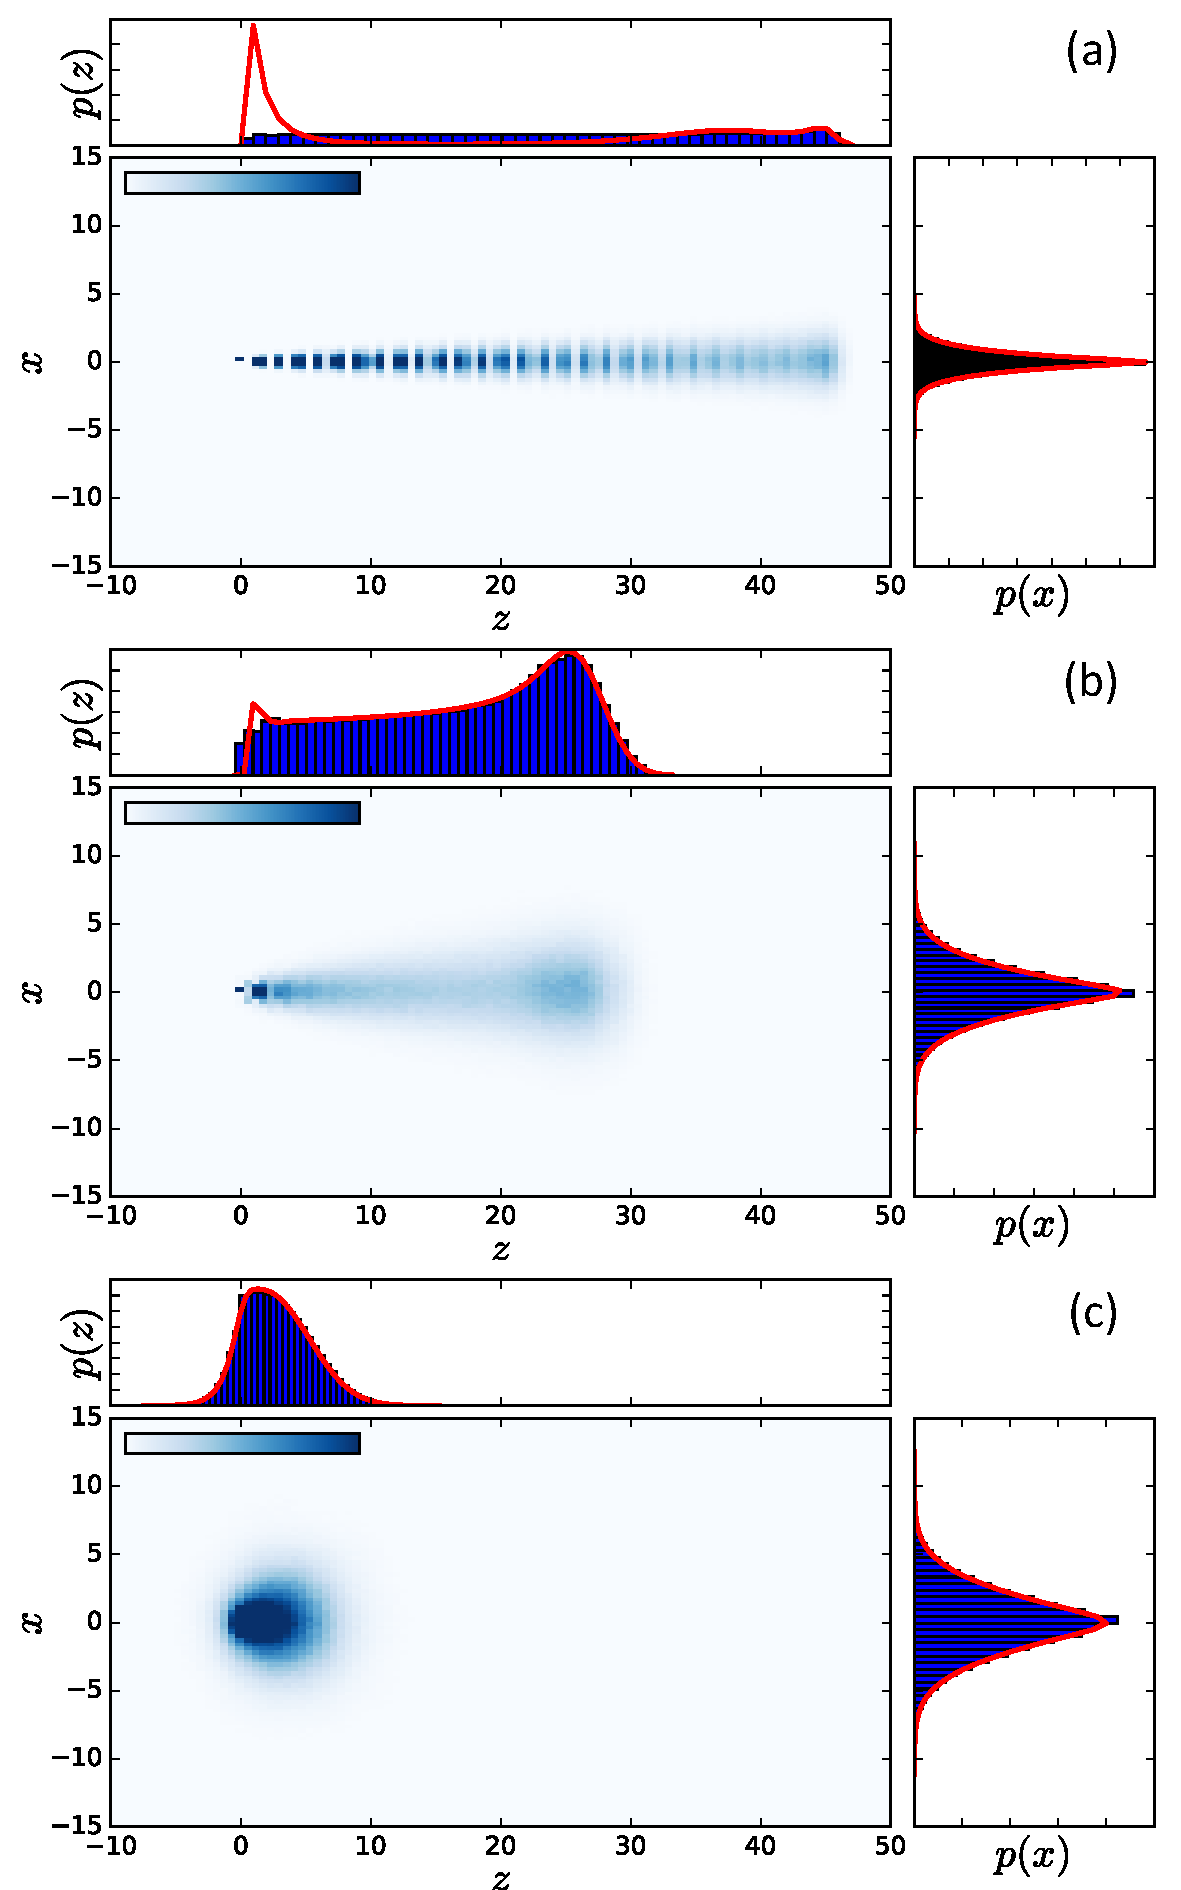
\includegraphics[width=0.9\linewidth]{shapeCases}
    \caption{The density distribution of pinned polymer shape for (a) strong external force field with $F=1$, (b) moderate external force field with $F=0.1$, (c) weak external force field with $F=0.01$. Other parameters are set as following $a=1,~k_B T = 1,~L=100$. See more explanations in the main text.}
    \label{fig:shapeCases}
\end{figure}

We show in Fig. \ref{fig:shapeCases} the monomer density distribution of a 3D pinned polymer loop projected in the 2D $x-z$ plane. 
The upper panel shows the marginal distribution of density along the force direction $z$ axis, while the right panel shows the marginal distribution of density perpendicular to the force direction along $x$ axis. The red lines represent the theoretical results which we will discuss next.

In section \ref{sec:equilibrium_statistics_in_3d}, we show the mean and variance of the bead position in 3D. When the dimensionless temperature is not too small ($\tilde{T}\gg 1$), the distribution of of the bead position can be considered as Gaussian. So we have
\begin{subequations}
    \label{eq:posDistribution}
    \begin{align}
    p(z_i) & = \frac{1}{\sqrt{2\pi \text{var}\left[z\right]_i}} \exp\left(-\frac{(z_i - \left<z_i\right>)^2}{2\text{var}\left[z_i\right]}\right), \\
    p(x_i) & = \frac{1}{\sqrt{2\pi \text{var}\left[x\right]_i}} \exp\left(-\frac{(x_i - \left<x_i\right>)^2}{2\text{var}\left[x_i\right]}\right).
    \end{align}
\end{subequations}
And then the marginal particle density can be calculated as
\begin{subequations}
    \label{eq:particleDensity}
    \begin{align}
        P(z) & = \frac{1}{L} \sum_{i=1}^L p(z_i), \\
        P(x) & = \frac{1}{L} \sum_{i=1}^L p(x_i).
    \end{align}
\end{subequations}
Substitute the mean and variance we obtained in section \ref{sec:equilibrium_statistics_in_3d}, the theoretical results of red lines in Fig. \ref{fig:shapeCases} can be obtained. Notice that the theory of $p(z)$ fits not so good with the simulation results in Fig. \ref{fig:shapeCases} (a), and it is because the Gaussian assumption is not valid in the strong force regime along the force direction. 

Although the density profile of monomers can be calculated as above, the intuition of the polymer shape is still unclear. In order to quantify the shape and get an intuition, we calculate the 3D gyration tensor of the polymer, which is defined as following:
\begin{equation}
    \label{eq:gyrationTensor}
    Q = \begin{bmatrix}
    Q_{xx} & Q_{xy} & Q_{xz} \\
    Q_{yx} & Q_{yy} & Q_{yz} \\
    Q_{zx} & Q_{zy} & Q_{zz} 
    \end{bmatrix}
    \rightarrow \begin{bmatrix}
    \lambda_{x}^2 & 0 & 0 \\
    0 & \lambda_{y}^2 & 0 \\
    0 & 0 & \lambda_{z}^2 
\end{bmatrix}
\end{equation}
where the elements $Q_{xy}$ can be written as 
\begin{equation}
    \label{eq:gyrationTensorElement}
    Q_{xy} = \frac{1}{L}\sum_{i=1}^L{(x_i-x_{CM})(y_i-y_{CM})},
\end{equation}
and $x_{CM}$ is the $x$ component of the center of mass vector. The right arrow in Eq.~\eqref{eq:gyrationTensor} means the diagonalization, and $\lambda_x^2, ~\lambda_y^2, ~\lambda_z^2$ represent the three non-negative eigenvalues of the gyration tensor. Physically, the intuition of the three eigenvalues can be interpreted as the magnitude of three orthogonal axes of the fitted ellipsoid enclosing the polymer loops. For convenience, we order them by $\lambda_x^2\leq\lambda_y^2\leq\lambda_z^2$.

Based on the gyration tensor, the first shape indicator we want to discuss is the gyration radius of the polymer, which is defined and can be calculated as following:
\begin{equation}
    \label{eq:gyrationRadius}
    R_g^2 :=  \frac{1}{L} \sum_{i=1}^L \left(\mathbf{r}_i - \mathbf{r}_{CM}\right)^2 = \lambda_x^2 + \lambda_y^2 + \lambda_z^2
\end{equation}

\begin{figure}[htpb]
    \centering
    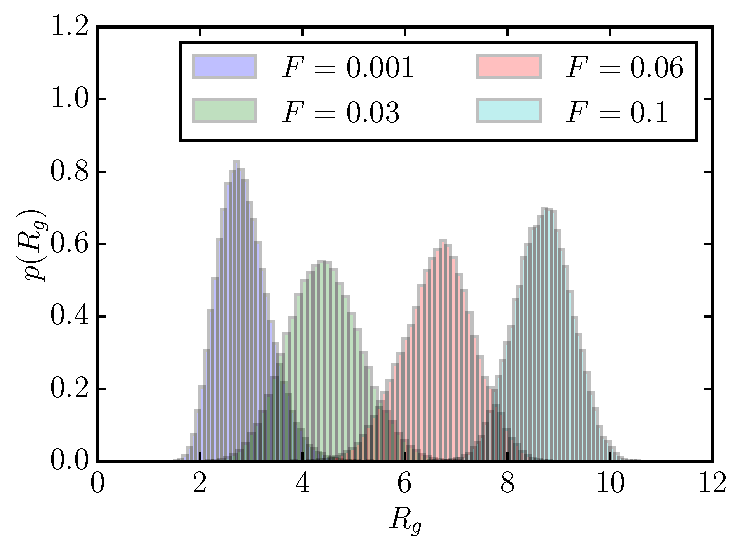
\includegraphics[width=0.8\linewidth]{rgpdf}
    \caption{The distribution of gyration radius of pinned polymer loop under different strength of external force field. $L=100, ~k_BT=1$. }
    \label{fig:rgpdf}
\end{figure}
In Fig. \ref{fig:rgpdf}, we show the distribution of gyration radius under several force field. Interestingly, we can see that the width of the distribution varies non-monotonically with the strength of external force. In other words, the gyration radius is more fluctuating under a moderate force field. 
The explanation for the unexpected non-monotonic behavior is the symmetry break because of the pinned effect. We can see in Fig. \ref{fig:shapeCases} (b) that the free end of the polymer is more fluctuating while the pinned end is fixed. This leads to a trumpet-like shape of the polymer. So we have the with of the distribution varies non-monotonically with the external fore field.

In next subsection, we will introduce two more descriptors of the polymer shape, which is the asphericity and the nature of asphericity.

\subsection{Asphericity and the nature of asphericity}
\label{sub:asphericity_and_the_nature_of_asphericity}

The asphericity and the nature of asphericity are two descriptors that commonly used to quantify the shape of the polymer. The definition of them are based on the gyration tensor \cite{Alim2007}. More specifically, the asphericity is defined by
\begin{equation}
    \label{eq:asphericity}
    \Delta = \frac{3}{2} \frac{\text{Tr}\hat{Q}^2}{(\text{Tr}Q)^2},
\end{equation}
where $\hat{Q}_{ij} = Q_{ij} - \delta_{ij}\text{Tr}Q/3$. The nature of asphericity is given by
\begin{equation}
    \label{eq:natureAsphericity}
    \Sigma = \frac{4\det\hat{Q}}{\left(\frac{2}{3}\text{Tr}\hat{Q}^2\right)^{3/2}}.
\end{equation}
However, in order to compare the shape of the pinned model with the researches in the literature \cite{Alim2007,Blavatska2010a}, we adopt the parameter $\rho = 2\sqrt{\Delta} \in [0,2]$ and $\theta = \arccos\Sigma/3\in[0,\pi/3]$. The physical interpretation of these parameters are illustrated in Fig. \ref{fig:shapeDistr} (a). Basically, $\rho=0$ corresponds to a fully spherical object while $\rho=2$ means the shape of the object is rod-like. And $\theta$ measures whether the object is prolate or oblate. 

\begin{figure}[htpb]
    \centering
    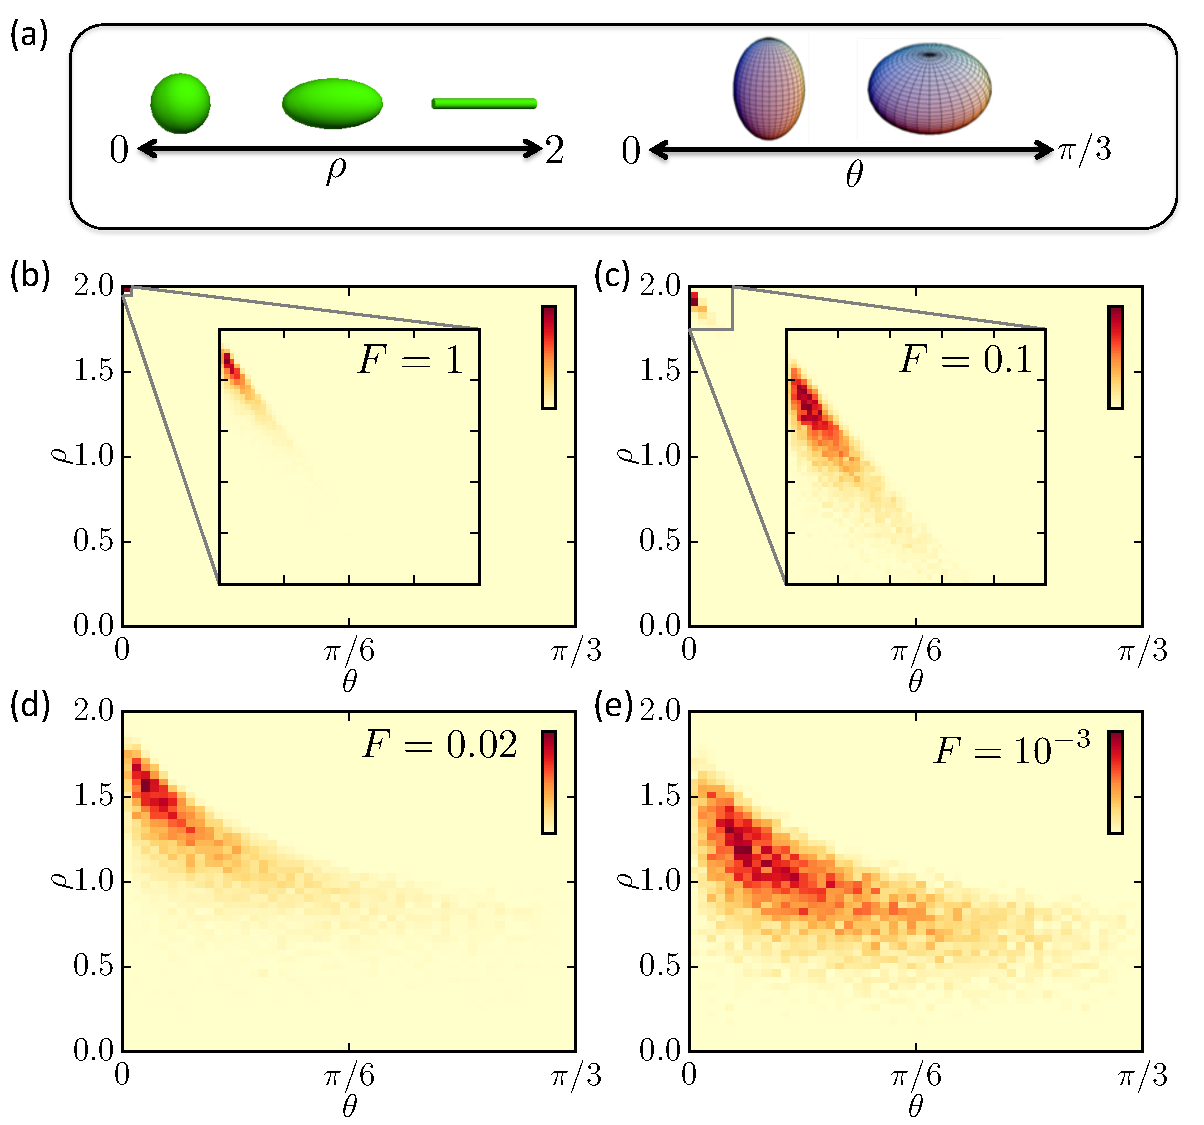
\includegraphics[width=1.0\linewidth]{shapeDistr}
    \caption{The shape of pinned polymer loop distributed over the phase diagram of asphericity and the nature of asphericity. (a) The intuition of asphericity and the nature of asphericity are illustrated. (b) The $\rho-\theta$ phase diagram for $F=1$. (c) The $\rho-\theta$ phase diagram for $F=0.1$. (d) The $\rho-\theta$ phase diagram for $F=0.02$. (e) The $\rho-\theta$ phase diagram for $F=0.001$. Other parameters such as $k_B T =1,~L=1,~a=1$.}
    \label{fig:shapeDistr}
\end{figure}

As we can see from Fig. \ref{fig:shapeDistr}, the shape of the pinned polymer loop is spread over a sickle-shaped area. In addition, the prolate and elongated shape is preferred no matter the external force is strong or not. The phase diagrams we found here are similar to those of semi-flexible unpinned polymer loops in \cite{Alim2007}.

In this section, we introduce several shape descriptors of pinned polymer loop based on the 3D gyration tensor. The theory monomer density distribution is also shown and compared to the Monte-Carlo simulation data and a good consistency is obtained. 



%********************************** % Sixth Section  *************************************
\section{Summary}
\label{sec:summary_chp3}

In this chapter, we discuss the equilibrium statistics of pined polymer loops in an external force field, which is our model for chromosomes in meiotic fission yeast. 

We first solve the statistics in a idealized 1D model. We introduce a technique which combines the \emph{Fermi-Dirac} statistics and Brownian Bridge condition to solve the problem in \emph{grand} canonical ensemble. The solution found is compared to the exact solution, which can be obtain after utilize the analogy to a number partition problem. However, we found that the results from our technique are quite accurate and the exact solution is quite cumbersome for later calculations. Thus the first approach is preferred. Using the result, we are able to calculate the mean and variance of bead position.  

And then we extend our theory to the three dimensional system. The same method of Brownian Bridge is used to solve the statistics. Also the three dimensional mean and variance of bead position is calculated. Moreover, the paring of polymer loops pinned at the same point is discussed. We calculate the statistical distance of the corresponding loci along the polymer loops. We found that the distance is reduced efficiently by the external force field. Thus the mechanism of facilitating pairing by pulling is illustrated. In addition, we also calculate the intersecting polymer loops in order to study the role of more constraints in the paring process. And the conclusion is additional constraints further reduce the fluctuation and facilitate the pairing. 

In the last section, we use our theoretical results to discuss the shape of pinned polymer loops in an external force field. The approximation for marginal distribution of monomer density is calculated in both parallel and transverse directions. And we quantify the shape based one the three dimensional gyration radius. Interestingly, we found the width of gyration radius distribution varies non-monotonic with the strength of the external force field. The phase diagram of asphericity and the nature of asphericity were shown which implies a rod-like and prolate shape of the pinned polymer loops in both weak and strong force field.

In next chapter, we will delve deeper to study the non-equilibrium properties of the pinned polymer loop polymer in an external force field. 
